    \documentclass[
        fleqn,
        usenatbib,
        referee,
    ]{mnras}
    \usepackage{
        amsmath,
        amssymb,
        newtxtext,
        newtxmath,
        ae, aecompl,
        graphicx,
        booktabs,
    }
    \usepackage[T1]{fontenc}
    \usepackage[
        labelfont=bf, % caption names are labeled in bold
        font=scriptsize % smaller font for captions
    ]{caption}
    \usepackage[caption=false]{subfig} % subfigures

    \newcommand*{\scinot}[2]{#1\times10^{#2}}
    \newcommand*{\rd}[2]{\frac{\mathrm{d}#1}{\mathrm{d}#2}}
    \newcommand*{\rtd}[2]{\frac{\mathrm{d}^2#1}{\mathrm{d}#2^2}}
    \newcommand*{\pd}[2]{\frac{\partial#1}{\partial#2}}
    \newcommand*{\ptd}[2]{\frac{\partial^2#1}{\partial#2^2}}
    \newcommand*{\md}[2]{\frac{\mathrm{D}#1}{\mathrm{D}#2}}
    \newcommand*{\at}[1]{\left.#1\right|}
    \newcommand*{\abs}[1]{\left|#1\right|}
    \newcommand*{\ev}[1]{\left\langle#1\right\rangle}
    \newcommand*{\p}[1]{\left(#1\right)}
    \newcommand*{\s}[1]{\left[#1\right]}
    \newcommand*{\z}[1]{\left\{#1\right\}}
    \newcommand*{\bm}[1]{\mathbf{#1}}
    \newcommand*{\uv}[1]{\hat{\mathbf{#1}}}
    \DeclareMathOperator*{\argmin}{argmin}
    \DeclareMathOperator*{\argmax}{argmax}
    \DeclareMathOperator*{\med}{med}
    \DeclareMathOperator*{\erf}{erf}

\title[Internal Gravity Wave Breaking in White Dwarf Binaries]{Internal Gravity
Wave Breaking in White Dwarf Binaries}
\author[Y. Su et\ al.]{
Yubo Su,$^1$,
Daniel Lecoanet,$^2$
Dong Lai,$^1$
\\
$^1$ Cornell Center for Astrophysics and Planetary Science, Department of
Astronomy, Cornell University, Ithaca, NY 14853, USA
\\
$^2$ Princeton Center for Theoretical Science, Princeton University, Princeton,
NJ 08544, USA
}

\date{Accepted XXX\@. Received YYY\@; in original form ZZZ}

\pubyear{2019}

\begin{document}\label{firstpage}
\pagerange{\pageref{firstpage}--\pageref{lastpage}}
\renewcommand*{\sectionautorefname}{Section}
\maketitle

% cp ../sims/agg.png plots; cp ../sims/2d_4_fourier/snapshots_lin_0_masked/f_amps.png plots/lin_amps.png; cp ../sims/2d_4_fourier/snapshots_lin_0_masked/fluxes.png plots/lin_fluxes.png; cp ../sims/2d_4_fourier/snapshots_yubo_nu1_vhres/f_amps.png plots/nl_f_amps.png; cp ../sims/2d_4_fourier/snapshots_yubo_nu1_vhres/fluxes.png plots/nl_fluxes.png; cp ../sims/2d_4_fourier/snapshots_yubo_nu1_vhres/f_refl.png plots/nl_f_refl.png; cp ../sims/2d_4_fourier/snapshots_yubo_nu1_vhres/f_ri.png plots/nl_f_ri.png; cp ../sims/2d_4_fourier/snapshots_yubo_nu1_vhres/front.png plots/nl_front.png;

\begin{abstract}
    In sufficiently compact white dwarf binaries, dynamical tides raise a train
    of internal gravity waves that propagate towards the surface and dissipate
    via nonlinear wave breaking. We perform 2D hydrodynamical simulations of
    this wave breaking in an incompressible, isothermal atmosphere. After an
    initial transient phase, we find that these waves generate a sharp
    transition, a critical layer, between the non-rotating core and
    synchronously rotating envelope. We find evidence that indefinite steepening
    of this critical layer is suppressed by the Kelvin-Helmholtz instability. We
    study the absorption and reflection of incident waves off the critical layer
    and provide analytical formulae describing its evolution. We infer
    necessary conditions to resolving momentum transfer within the critical
    layer. Finally, we speculate on the application of our model to tidal
    synchronization and heating in astrophysical systems.
\end{abstract}

\begin{keywords}
white dwarfs -- hydrodynamics -- binaries:close -- waves % chktex 8
\end{keywords}

\section{Introduction}

Compact white dwarf (WD) binary systems, with orbital periods in the range of
minutes to hours, are important for a range of astrophysical problems. They are
the most important sources of gravitational waves (GWs) for the Laser
Interferometric Space Antenna (LISA) \citep{lisa}. They are also thought to
produce interesting optical transients such as underluminous supernovae
\citep{underlum}, Ca-rich fast transients \citep{carich}, and tidal novae
\citep{tidal_novae}. Most importantly, they have been proposed as the likely
progenitors of type Ia supernovae (e.g. \citealp{Ia0,webbink} or more recently
\citealp{Ia1,Ia2}). While presently only a few tens of compact WD binaries are
known \citep{lsst_wd}, \emph{Gaia} (currently gathering data) is expected to
expand the catalog to a few hundreds \citep{lsst_wd} \citep[results based on
\emph{Gaia}'s second data release have already begun to
appear][]{gaiaDD,gaiaDD2}, and the Large Synoptic Survey Telescope (LSST, first
light scheduled for 2020) will likely detect a few thousand more
\citep{lsst_wd}. These observations will significantly advance the understanding
of WD binaries and their evolution.

In spite of the broad importance of WD binaries, the evolution of these systems
prior to their final mergers is not well understood. Much of this uncertainty
comes from our imprecise understanding of tidal interactions, which play an
important role during a compact WD binary's inspiral \citep{fullerII}. Previous
studies have shown that these interactions manifest as tidal excitation of
internal gravity waves (IGW), waves in the WD fluid restored by the buoyancy
force due to density stratification \citep{fullerI}. As these waves propagate
outwards towards the WD surface, they grow in amplitude until they break, as do
ocean waves on a shore, and transfer both energy and angular momentum from the
binary orbit to the outer envelope of the WD \citep{fullerI,fullerII}.

Previous works have found that the dissipation of IGW can generate significantly
more energy than thermal radiation from the isolated WD surface and is thus a
major contributor to the WD energy budget \citep{fullerII,fullerIV}. However,
these works parameterized the wave breaking process in an ad hoc manner. The
details of dissipation, namely the location and spatial extent of the wave
breaking, affect the observable outcome: dissipation near the surface of the WD
can be efficiently radiated away and simply brightens the WD, while dissipation
deep in the WD envelope causes an energy buildup that results in energetic
flares \citep{tidal_novae}. Works in other fields based on numerical simulations
show that strongly nonlinear wave breaking behaves differently than predictions
based in linear and weakly nonlinear theory \citep{winters1994,barker_ogilvie}.
Such fully nonlinear numerical simulations have not been performed for WDs.

In this paper, we perform numerical simulations of tidally-excited IGWs
undergoing wave breaking in an idealized WD fluid. The primary aim of the paper
is to thoroughly characterize the angular momentum transfer within a WD by
purely hydrodynamical effects. As a first approximation, we analyze the problem
in a 2D Cartesian geometry, and consider IGW propagating into a fluid initially
at rest. We find that, after an initial transient phase, the fluid develops two
distinct zones: (i) a lower zone that has no horizontal mean flow, and (ii) an
upper zone with significant horizontal mean flow.

These two zones are separated by a \emph{critical layer}. The majority of our
paper is dedicated to characterizing the behavior of the critical layer when
interacting with a continuous train of IGW excited from the bottom of the fluid.
IGW are generally \emph{anti}-diffusive, in that they steepen shear flows
\citep{lindzen_qbo,lecoanet_meanflow}, and act to narrow the critical layer. We
find this steepening is suppressed by the Kelvin-Helmholtz instability and
turbulence within the very narrow critical layer. By careful accounting of the
momentum flux budget about the critical layer, we are able to model the
propagation of the critical layer, reflection of the incident IGW, and other
momentum redistribution behaviors. Our results are numerically converged
for sufficiently large resolutions.

In \autoref{s:equations}, we will describe the system of equations we will use
to analyze IGW breaking. In \autoref{s:theory}, we review existing understanding
of wave breaking and present new analytical results. In \autoref{s:numerics}, we
describe our numerical setup, which in \autoref{s:weak_sim} we validate in the
weak forcing limit against linear theory. In \autoref{s:sim}, we present the
results of simulation of IGW breaking and our characterization of the critical
layer. Finally, we summarize and conclude in \autoref{s:discussion}.

\section{Problem Description}\label{s:equations}

We consider a incompressible, isothermal fluid, representative of degenerate
matter in WDs. We use barotropic equation of state $P(\rho, T) = P(\rho)$ as a
first approximation. As we are interested in dynamics far from the center of the
WD, we approximate the gravitational field as uniform. We model the background
density stratification as $\overline{\rho} = \overline{\rho}_0 e^{-z/H}$ for
some reference density $\overline{\rho}_0$ (we generally notate background
quantities with overbars and perturbation quantities with primes). We
consider a 2D fluid with for computational feasibility. While
it is well-known wave breaking is a 3D process \citep{klostermeyer,winters1994},
the dynamical effect of the breaking process is likely to be similar in 2D
\citep{barker_ogilvie}. Finally, we simplify by considering simple
plane-parallel IGW\@. Since wave breaking generally occurs near the surface of
WDs \citep[$\gtrsim 0.9R_{WD}$][]{fullerI}, the curvature of the wave front is
negligible.

The Euler equations for an incompressible, barotropic fluid in a uniform
gravitational field are
\begin{subequations}\label{se:nl_orig}
    \begin{align}
        \bm{\nabla} \cdot \bm{u} &= 0,\label{eq:nl_incomp}\\
        \md{\rho}{t} &= 0 ,\label{eq:nl_density}\\
        \md{\bm{u}}{t} + \frac{\bm{\nabla}P}{\rho} + g\uv{z} &=
            0\label{eq:nl_mom}.
    \end{align}
\end{subequations}
$\md{}{t} = \pd{}{t} + \p{\bm{u} \cdot \bm{\nabla}}$ is the Lagrangian or
material derivative, and $\bm{u}, \rho, P$ denote the velocity field, density
and pressure respectively. We denote $-g\uv{z}$ constant gravitational
acceleration. Note that at hydrostatic equilibrium $\pd{}{t} = 0$ we have
$\bm{\nabla}\overline{P} = -\overline{\rho} g\uv{z}$ and so $\overline{P} =
\overline{\rho} gH$. A vertically-stratified shear flow
$\overline{u}_x(z)\uv{x}$ is permitted at hydrostatic equilibrium, but we will
assume no background flow, so $\bm{u} = \bm{u}'$. Physically, this assumption
corresponds to a non-rotating star, or going to the corotating frame of a
rigidly rotating star.

In practice, it is convenient to introduce the coordinate $\Upsilon = \ln
\frac{\rho}{\overline{\rho}}$ \citep[e.g.][]{lecoanet_anel}. This both
identically enforces $\rho > 0$ and eliminates the stiff term
$\frac{\bm{\nabla}P}{\rho}$. We also define reduced pressure $\varpi =
\frac{P}{\rho}$. Then, we may rewrite the second two equations of
\autoref{se:nl_orig} as
\begin{subequations}\label{se:nl_upsilon}
    \begin{align}
        \md{\Upsilon}{t} + u_z \pd{\ln \overline{\rho}}{z} &= 0
            ,\label{eq:nl_up_density} \\
        \md{\bm{u}}{t} + \bm{\nabla}\varpi + \varpi\bm{\nabla}\Upsilon
            - \frac{\varpi}{H}\uv{z} + g\uv{z} &= 0\label{eq:nl_upsilon_u}.
    \end{align}
\end{subequations}
In the new coordinates, hydrostatic equilibrium corresponds to $\Upsilon = 0,
\overline{\varpi} = gH$.

\section{Internal Gravity Waves: Theory}\label{s:theory}

\subsection{Linear Analysis}

In the small perturbation limit, where flow velocities are small compared to the
characteristic space and time scales $\pd{}{t} \gg \bm{u} \cdot
\bm{\nabla}$, we may linearize \autoref{se:nl_upsilon}. The solution in this
linear regime is given by \citep{drazin,sutherland0}:
\begin{equation}
    u_z\p{x, z, t} = Ae^{z/2H}\cos\p{k_{x}x + k_{z}z - \omega t},
        \label{eq:k0z_sign}
\end{equation}
where $A$ is the amplitude and $\omega$ satisfies dispersion relation
\begin{equation}
    \omega^2 = \frac{N^2k_{x}^2}{k_{x}^2 + k_{z}^2 + \frac{1}{4H^2}}.
        \label{eq:disp_rel}
\end{equation}
Our equations are valid in the limit of large sound speed $c_s \to \infty$, in
which the \emph{Brunt-V\"ais\"al\"a frequency}
\begin{equation}
    N^2 \equiv g^2\p{\rd{\rho}{P} - \frac{1}{c_s^2}} = \frac{g}{H},
\end{equation}
is constant. Other dynamical quantities are simply related to $u'_z$ \citep[see
e.g.][]{sutherland0}.

In the short-wavelength/WKB limit $\abs{k_{z}H} \gg 1$, the solution exhibits
the following characteristics:
\begin{itemize}
    \item The amplitude of the wave grows with $z$ as $e^{z/2H}$. Thus, the
        linear approximation is always violated for sufficiently large $z$.

    \item The phase and group velocities are respectively:
        \begin{align}
            \bm{c}_{p} &=
                \p{k_{x}\uv{x} + k_{z}\uv{z}}\frac{\omega}
                {k_{x}^2 + k_{z}^2 + \frac{1}{4H^2}},\\
            \bm{c}_{g} &= N\frac{\p{k_{z}^2 + \frac{1}{4H^2}}\uv{x}
                - \p{k_{x}k_{z}\uv{z}}}
                {\p{k_{x}^2 + k_{z}^2 + \frac{1}{4H^2}}^{3/2}}.\label{eq:vg}
        \end{align}
        We note $\bm{c}_{p} \cdot \bm{c}_g = \mathcal{O}\p{ \p{k_{z}H}^{-2} }
        \approx 0$. In the Boussinesq approximation where density stratification
        outside of $N^2$ is completely neglected, the phase and group velocity
        are exactly orthogonal \citep{drazin,sutherland1}. We use the convention
        where upward propagating IGW have $c_{g, z} > 0$, $k_z < 0, k_x > 0$.

    \item The averaged horizontal momentum flux $F$ is
        \begin{align}
            F &\equiv \ev{\rho u_{x} u_{z}}_x \equiv
                \frac{1}{L_x}\int_0^{L_x}\limits \rho u_{x}u_{z}\;\mathrm{d}x,
                    \label{eq:F_def}\\
                &\approx -\frac{A^2}{2}\overline{\rho}_0\frac{k_{z}}{k_{x}},
                    \label{eq:S_lin}
        \end{align}
        Thus, indeed $F > 0$ for an upward propagating IGW $c_{g, z} > 0$.
\end{itemize}

\subsection{Wave Generation}

To model continuous excitation of IGWs deep in the WD interior propagating
towards the surface, we use a volumetric forcing term to excite IGW near the
bottom of the simulation domain. Our forcing excites both IGWs
propagating upwards, imitating a wave tidally excited deeper in the WD, and
downwards, which are not physically meaningful, but are damped away by the
damping layers described in \autoref{ss:damping}.

As not to interfere with the incompressibility constraint, we force the system
on the density equation. We implement forcing with strength $C$ localized around
$z_0$ with small width $\sigma$ by replacing \autoref{eq:nl_up_density} with
\begin{equation}
    \md{\Upsilon}{t} + u_{z}\pd{\ln \overline{\rho}}{z}
        = Ce^{-\frac{(z - z_0)^2}{2\sigma^2}}
            \cos \p{k_{x}x - \omega t}.\label{eq:vol_drive}
\end{equation}
Using a narrow Gaussian profile excites a broad $z$ power spectrum, but only the
$k_{z}$ satisfying dispersion relation \autoref{eq:disp_rel} for the given
$k_{x}$, $\omega(k_{x}, k_{z})$ will propagate.

In the linearized system, the effect of this forcing can be solved exactly
(\autoref{s:force_solved}). If we approximate $k_zH \gg 1, \sigma \ll H$, the
solution can be approximated as two plane waves propagating away from the
forcing zone
\begin{align}
    u_{z}&(x, z, t) \approx{} \frac{C}{2k_z}\frac{gk_x^2}{\omega^2}
        e^{-\frac{k_z^2\sigma^2}{2}}
        \sqrt{2\pi \sigma^2} \times\nonumber\\
        &{}\begin{cases}
        e^{\frac{z - z_0}{2H}}\sin\p{k_{x}x + k_{z}(z - z_0) - \omega t
            + \frac{k_z\sigma^2}{2H}}
            & z > z_0\\
        e^{\frac{z - z_0}{2H}}\sin\p{k_{x}x - k_{z}(z - z_0) - \omega t
            + \frac{k_z\sigma^2}{2H}}
            & z < z_0\\
    \end{cases}.\label{eq:uz_lin}
\end{align}
The $z > z_0$ region models an upward propagating IGW wavetrain excited deep
in the atmosphere.

\subsection{Wave Breaking Height}\label{ss:wave_breaking}

Above, we neglected advective terms $\pd{}{t} \gg \bm{u} \cdot \bm{\nabla}$.
However, since $\abs{\bm{u}} \propto e^{z/2H}$ in an infinite domain all IGWs
eventually grow to nonlinear amplitudes and break. Nonlinear wave breaking is
expected to be important in WDs \citep{fullerI,fullerII}. We can
estimate the height of wave breaking using $\frac{\abs{\bm{u}}
\abs{\bm{k}}}{\omega} \sim 1$. This can be rewritten using the Lagrangian
displacement $-i\omega \bm{\xi} = \bm{u}$:
\begin{equation}
    \xi_z k_z \gtrsim 1.\label{eq:nl}
\end{equation}

% An equivalent estimate given by \citep{eliassen_palm_cite,sutherland0} is that
% IGWs break when the wave-induced mean flow is equal to the horizontal phase
% velocity
% \begin{equation}
%     \overline{U}(z) = \frac{\ev{u_{x}u_{z}}_x}{c_{g,z}} \sim
%         \frac{\omega}{k_x},\label{eq:rip}
% \end{equation}
% where \overline{U}(z) \equiv \ev{u_x}_x$ is the mean flow of the fluid.
% \autoref{eq:rip} provides a leading-order estimate for \overline{U}(z)$ which
% may further evolve over time (see \autoref{ss:crit_layer}); for a general mean
% flow, \autoref{eq:rip} also defines the criterion for a \emph{critical
% layer}. This wave-induced mean flow is analogous to Stokes' drift for surface
% waves and can be derived by considering the propagation of $F$
% (\autoref{eq:F_def}) into a medium at rest. Evaluating \autoref{eq:rip}
% yields agreement with \autoref{eq:nl}.


\citealp{drazin, klostermeyer, winters1994} describe the onset of wave breaking.
At intermediate amplitudes, wave breaking occurs via triadic resonances which
transfer energy from the ``parent’’ internal gravity wave (in our problem, the
tidally forced wave) to ``daughter’’ internal gravity waves on smaller length
scales that efficiently damp. The horizontal momentum flux decreases from $F$ to
$0$ over this breaking region. The lost flux is deposited into a horizontal mean
flow
\begin{equation}
    \overline{U}(z, t) \equiv \ev{u_x}_x.\label{eq:mean_flow}
\end{equation}
As the mean flow grows, a \emph{critical layer} may form, discussed below.

\subsection{Critical Layers}\label{ss:crit_layer}

A horizontal shear flow $\overline{U}(z, t)\hat{x}$ enters the fluid equations
via the Lagrangian derivative, which can be decomposed as
\begin{equation}
    \md{}{t} = \pd{}{t} + \overline{U} \pd{}{x} + \p{\bm{u}' \cdot \vec{\nabla}},
\end{equation}
where $\bm{u}'$ is the velocity field \emph{without} the shear flow, for
clarity. Thus, $\overline{U}$ has the effect of Doppler shifting the time
derivative into the frame comoving with the mean flow. If $\overline{U}$ is
roughly constant, then the behavior of a small plane wave perturbation satisfies
modified dispersion relation
\begin{equation}
    \p{\omega - \overline{U}k_x}^2 =
        \frac{N^2k_{x}^2}{k_{x}^2 + k_{z}^2 + \frac{1}{4H^2}}.
        \label{eq:disp_rel_U}
\end{equation}
This is just \autoref{eq:disp_rel} with $\omega \to \omega - \overline{U}k_x$.
It is apparent that if $\overline{U} = \overline{U}_c$, where
\begin{equation}
    \overline{U}_c \equiv \frac{\omega}{k_x},
\end{equation}
then the dispersion relation is singular and the linear solution breaks down.
Physically, this corresponds to the Doppler-shifted frequency of the IGW being
zero. Anywhere $\overline{U} = \overline{U}_c$ is called a \emph{critical
layer}.

The behavior of an IGW incident upon a critical layer was first studied in the
inviscid, linear regime in \citealp{booker_bretherton}, which found nearly
complete absorption of the IGW\@. In particular, the incident wave has amplitude
reflection and transmission coefficients that can be expressed in terms of the
local Richardson number Ri at the height of the critical layer $z_c$:
\begin{align}
    \mathrm{Ri} &\equiv \at{\frac{N^2}{\p{\pd{\overline{U}}{z}}^2}}_{z_c},
        \label{eq:ri_def}\\
    \mathcal{R}_A &= e^{-2\pi \sqrt{\mathrm{Ri} - \frac{1}{4}}}, &
    \mathcal{T}_A &= e^{-\pi \sqrt{\mathrm{Ri} - \frac{1}{4}}}.
        \label{eq:crit_coeffs}
\end{align}
In the $\mathrm{Ri} \gg 1$ limit, $\mathcal{R}, \mathcal{T} \ll 1$
and the incident wave is completely absorbed to a good approximation.

This result extends to viscous fluids \citep{hazel}, but weakly nonlinear theory
\citep{brown_stewartson} and numerical simulations \citep{winters1994} suggest
that nonlinear effects may significantly enhance reflection and transmission.
Understanding the interaction of IGW and critical layers has important
applications: it is thought to be responsible for tidal synchronization in
stellar binaries \citep{zahn75,gn89} as well as terrestrial phenomena such as
the quasi-biennial oscillation \citep{lindzen_qbo}.

Consider the horizontal momentum transfer at the critical layer. Any incident
horizontal momentum flux absorbed by the fluid must manifest as additional
horizontal momentum of the shear flow. Since $\overline{U}$ cannot exceed
$\overline{U}_c$, the critical layer will instead propagate downward in response
to the incident momentum flux. The horizontal momentum of the shear flow
satisfies
\begin{equation}
    \pd{}{t}\int\limits \overline{\rho}(z) \overline{U}(z, t)\;\mathrm{d}z
        - F_a(t) = 0,
\end{equation}
where $F_a(t) > 0$ is the absorbed horizontal momentum. Assuming $\overline{U}(z
> z_c) = \overline{U}_c, \overline{U}(z < z_c) = 0$, this condition becomes
\begin{equation}
    \overline{\rho}(z_c) \overline{U}_c\rd{z_c}{t} = F_a(t).\label{eq:zc_anal}
\end{equation}
If $F_a$ is constant in time, $z_c(t)$ has analytical solution
\begin{equation}
    z_c(t) = -H\ln \s{e^{-\frac{z_c(t = 0)}{H}} +
        \frac{tF_a}{\overline{U}_c H\overline{\rho}_0}},\label{eq:zc_sol}
\end{equation}
where $z_c(t = 0)$ is the initial critical layer height.

\section{Numerical Simulation Setup}\label{s:numerics}

We verify the analytic theory of \autoref{s:theory} by running weakly forced
direct numerical simulations using the pseudo-spectral code Dedalus
\citep{dedalus,dedalus2}. IGWs are excited deep within WDs and must propagate
across many density scale heights before reaching the surface. The waves stay
linear until they are within a few scale heights of the breaking height. We thus
simulate only the upper part of the WD\@. Although turbulence driven by wave
breaking is fundamentally 3D \citep{klostermeyer}, we simplify the problem by
restricting our simulations to two dimensions. Future work will study the
problem in 3D spherical geometry.

\subsection{Parameter Choices}

We simulate equations \autoref{eq:nl_incomp}, \autoref{eq:nl_upsilon_u}, and
\autoref{eq:vol_drive} in a Cartesian box with size $L_x, L_z$. The $x$
direction represents the azimuthal direction in a star, and the $z$ direction
represents the radial direction. We thus choose periodic boundary conditions in
the $x$ direction. We also use periodic boundary conditions in the $z$
direction, but we damp perturbations to zero near the top/bottom of the domain
to capture their distinct behavior (described in \autoref{ss:damping}). We
expand all variables as Fourier series with $N_x$ and $N_z$ modes, and use the
$3/2$ dealiasing rule to avoid aliasing errors in the nonlinear terms
\citep{boyd}.

The geometry of our simulation domain is fixed by one further parameter: $z_0$
the forcing location. We choose $L_z = 12.5H$ to give $\sim e^3$ amplitude growth
between the damping zones. We force at $z_0 = 3H$ within width $\sigma =
0.078H$, sufficiently far from the lower damping zone and permit sufficient room
for the upward moving wave to grow as $\propto e^{z/2H}$. Finally, we want
similar grid spacing $\frac{L_x}{N_x} \sim \frac{L_z}{N_z}$, guided by the
intuition that turbulence is approximately isotropic, so we use $L_x = 4H$ and
$N_z / N_x = 4$.

The time integration uses a split implicit-explicit third-order scheme where
certain terms are treated implicitly and the remaining terms are treated
explicitly. A third-order, four-stage DIRK-ERK scheme \citep{ascher} is used
with adaptive timesteps computed from advective Courant-Friedrichs-Lewy (CFL)
time. Specifically, we use $\Delta t = 0.7 \min(\Delta x / u_x,\Delta z /
u_{z})$, where the minimum is taken over every grid point in the domain and
$\Delta x,\Delta z$ are the grid spacings in the $x$ and $z$ directions
respectively.

We non-dimensionalize the problem such that $H = N = \rho_0 = 1$. The physics of
the simulation is then fixed by the four remaining parameters $k_{x}, \omega, C,
\nu$. We describe our choices for these parameters below:
\begin{itemize}
    \item $k_{x}$: Tidally excited waves in stars generally have $\ell = 2$,
        corresponding to a very small $k_\perp\sim 1/R$, where $R$ is the radius
        of the star. We use the smallest wavenumber in our simulation,
        $k_x=2\pi/L_x$.

    \item $\omega$: We choose $\omega$ by evaluating the dispersion relation
        $\omega(k_x, k_z)$ for a desired $k_z$. We pick $\abs{k_z H} = 2\pi$ to
        ensure the waves are very well resolved in all of our simulations. Note
        however that tidally forced IGWs typically have $\omega \ll N$, or
        equivalently $k_r/k_\perp \sim k_r R \gg 1$. This requires $k_z H
        \gtrsim 1$, which is only marginally satisfied in our simulations.

    \item $C$: In our weak forcing simulations, we first choose $C$ forcing
        strength such that $\xi_z k_z \ll 1$ is satisfied everywhere in the
        simulation domain. This constrains $C$ by \autoref{eq:uz_lin}.

    \item $\nu$: Nonlinear effects transfer wave energy from the injection
        wavenumber $\bm{k}$ to larger wavenumbers. Our spectral method does not
        have any numerical viscosity, so diffusivity must be introduced into the
        equations to regularize the systems at large wavenumbers. We add
        viscosity and diffusivity to the system in a way that conserves
        horizontal momentum (see Appendix~\ref{se:strat_impl} for details).

        To quantify $\nu$, we define the dimensionless Reynolds number
        \begin{equation}
            \mathrm{Re}  \equiv \frac{\omega}{\nu k_{z}^2}. \label{eq:re_def}
        \end{equation}
        When the forcing is weak, we may set $\nu \approx 0$, or $\mathrm{Re}
        \gg 1$ because there is negligible energy transfer between modes. Note
        that $\nu = 0$ exactly changes the order of the PDE system, as the
        highest-order derivatives appear only in the dissipitive terms, so a
        nonzero $\nu$ must be chosen even in linear simulations.
\end{itemize}

Finally, we use initial conditions $\bm{u}(x, z, 0) = \Upsilon(x, z, 0) = 0,
\varpi(x, z, 0) = 1$ corresponding to hydrostatic equilibrium and no initial
fluid motion.

\subsection{Damping Layers}\label{ss:damping}

We aim to damp waves that reach the edge of the simulation domain without
inducing nonphysical reflection. To do so, we replace material derivatives
in \autoref{se:nl_upsilon} with:
\begin{align}
    \md{}{t} &\to \md{}{t} + \Gamma(z),\\
    \Gamma(z) &= \frac{1}{2\tau}\s{2 + \tanh \frac{z - z_T}{\Delta z}
        + \tanh \frac{z_B - z}{\Delta z}},\label{eq:Gamma}
\end{align}
where $z_B = 1.5H, z_T = 10.5H$ are the boundaries of the damping zone.
This strongly damps perturbations below $z_B$ and above $z_T$ with damping time
$\tau$, negligibly affects dynamics between $z_B, z_T$ and has transition width
governed by $\Delta z$. We use $\Delta z = 0.25H$ and $\tau = 1/15N$. This
prescription is similar to \citep{lecoanet_damp} and has the advantage of being
smooth, important for spectral methods. Further details of our implementation of
the fluid equations in Dedalus are described in Appendix~\ref{se:strat_impl}.

\section{Weakly Forced Numerical Simulation}\label{s:weak_sim}

We describe the results of a simulation with $C = \scinot{1.64}{-7}$ such that
$\xi_z k_z \ll 1$ everywhere. In particular, $\xi_z k_z \approx \scinot{5}{-5}$
just above the forcing zone. A nonzero $\nu$ corresponding to $\mathrm{Re} =
10^7$ was used.

We expect the waves to follow the solution given by \autoref{eq:uz_lin}. Along
with incompressibility (\autoref{eq:nl_incomp}), we obtain a complete analytical
solution for flow velocities $\bm{u}_{al}(x, z, t)$. The amplitude of the
observed IGW in the simulation field $\bm{u}$ relative to analytical solution
$\bm{u}_{al}$ over some region $z \in [z_b, z_t]$ can be estimated with
\begin{equation}
    A_i(t) = \frac{\int\limits_{z_b}^{z_t}\int\limits_0^{L_x}
        \overline{\rho}\p{\bm{u} \cdot \bm{u}_{al}}\;\mathrm{d}x\mathrm{d}z}
        {\int\limits_{z_b}^{z_t}\int\limits_0^{L_x}
        \overline{\rho}\abs{\bm{u}_{al}}^2\;\mathrm{d}x\mathrm{d}z}
        \label{eq:ahat_def}
\end{equation}
The subscript $i$ denotes the incident wave. If $\bm{u} = \bm{u}_{al}$, then
$A_i(t) = 1$. The normalization is chosen such that the overlap between $\bm{u},
\bm{u}_{al} \propto e^{z/2H}$ is evenly weighted throughout the integration
region.

For a simulation satisfying $\xi_z k_z \ll 1$ everywhere, we expect
$A_i(t) = 1$ when integrated between the forcing and damping zones, i.e.\
$z_b \gtrsim z_0, z_t \lesssim z_T$ ($z_0, z_T$ are defined in
\autoref{eq:vol_drive} and \autoref{eq:Gamma} respectively). For consistency
with the nonlinear case later, we choose $z_b = z_0 + 3\sigma, z_t = z_b + H$
(using $z_t = z_T - \Delta z$ just below the damping layer instead does not
change the results). The resulting measurement of $A_i(t)$ is shown in
\autoref{fig:lin_amps}.
\begin{figure}
    \centering
    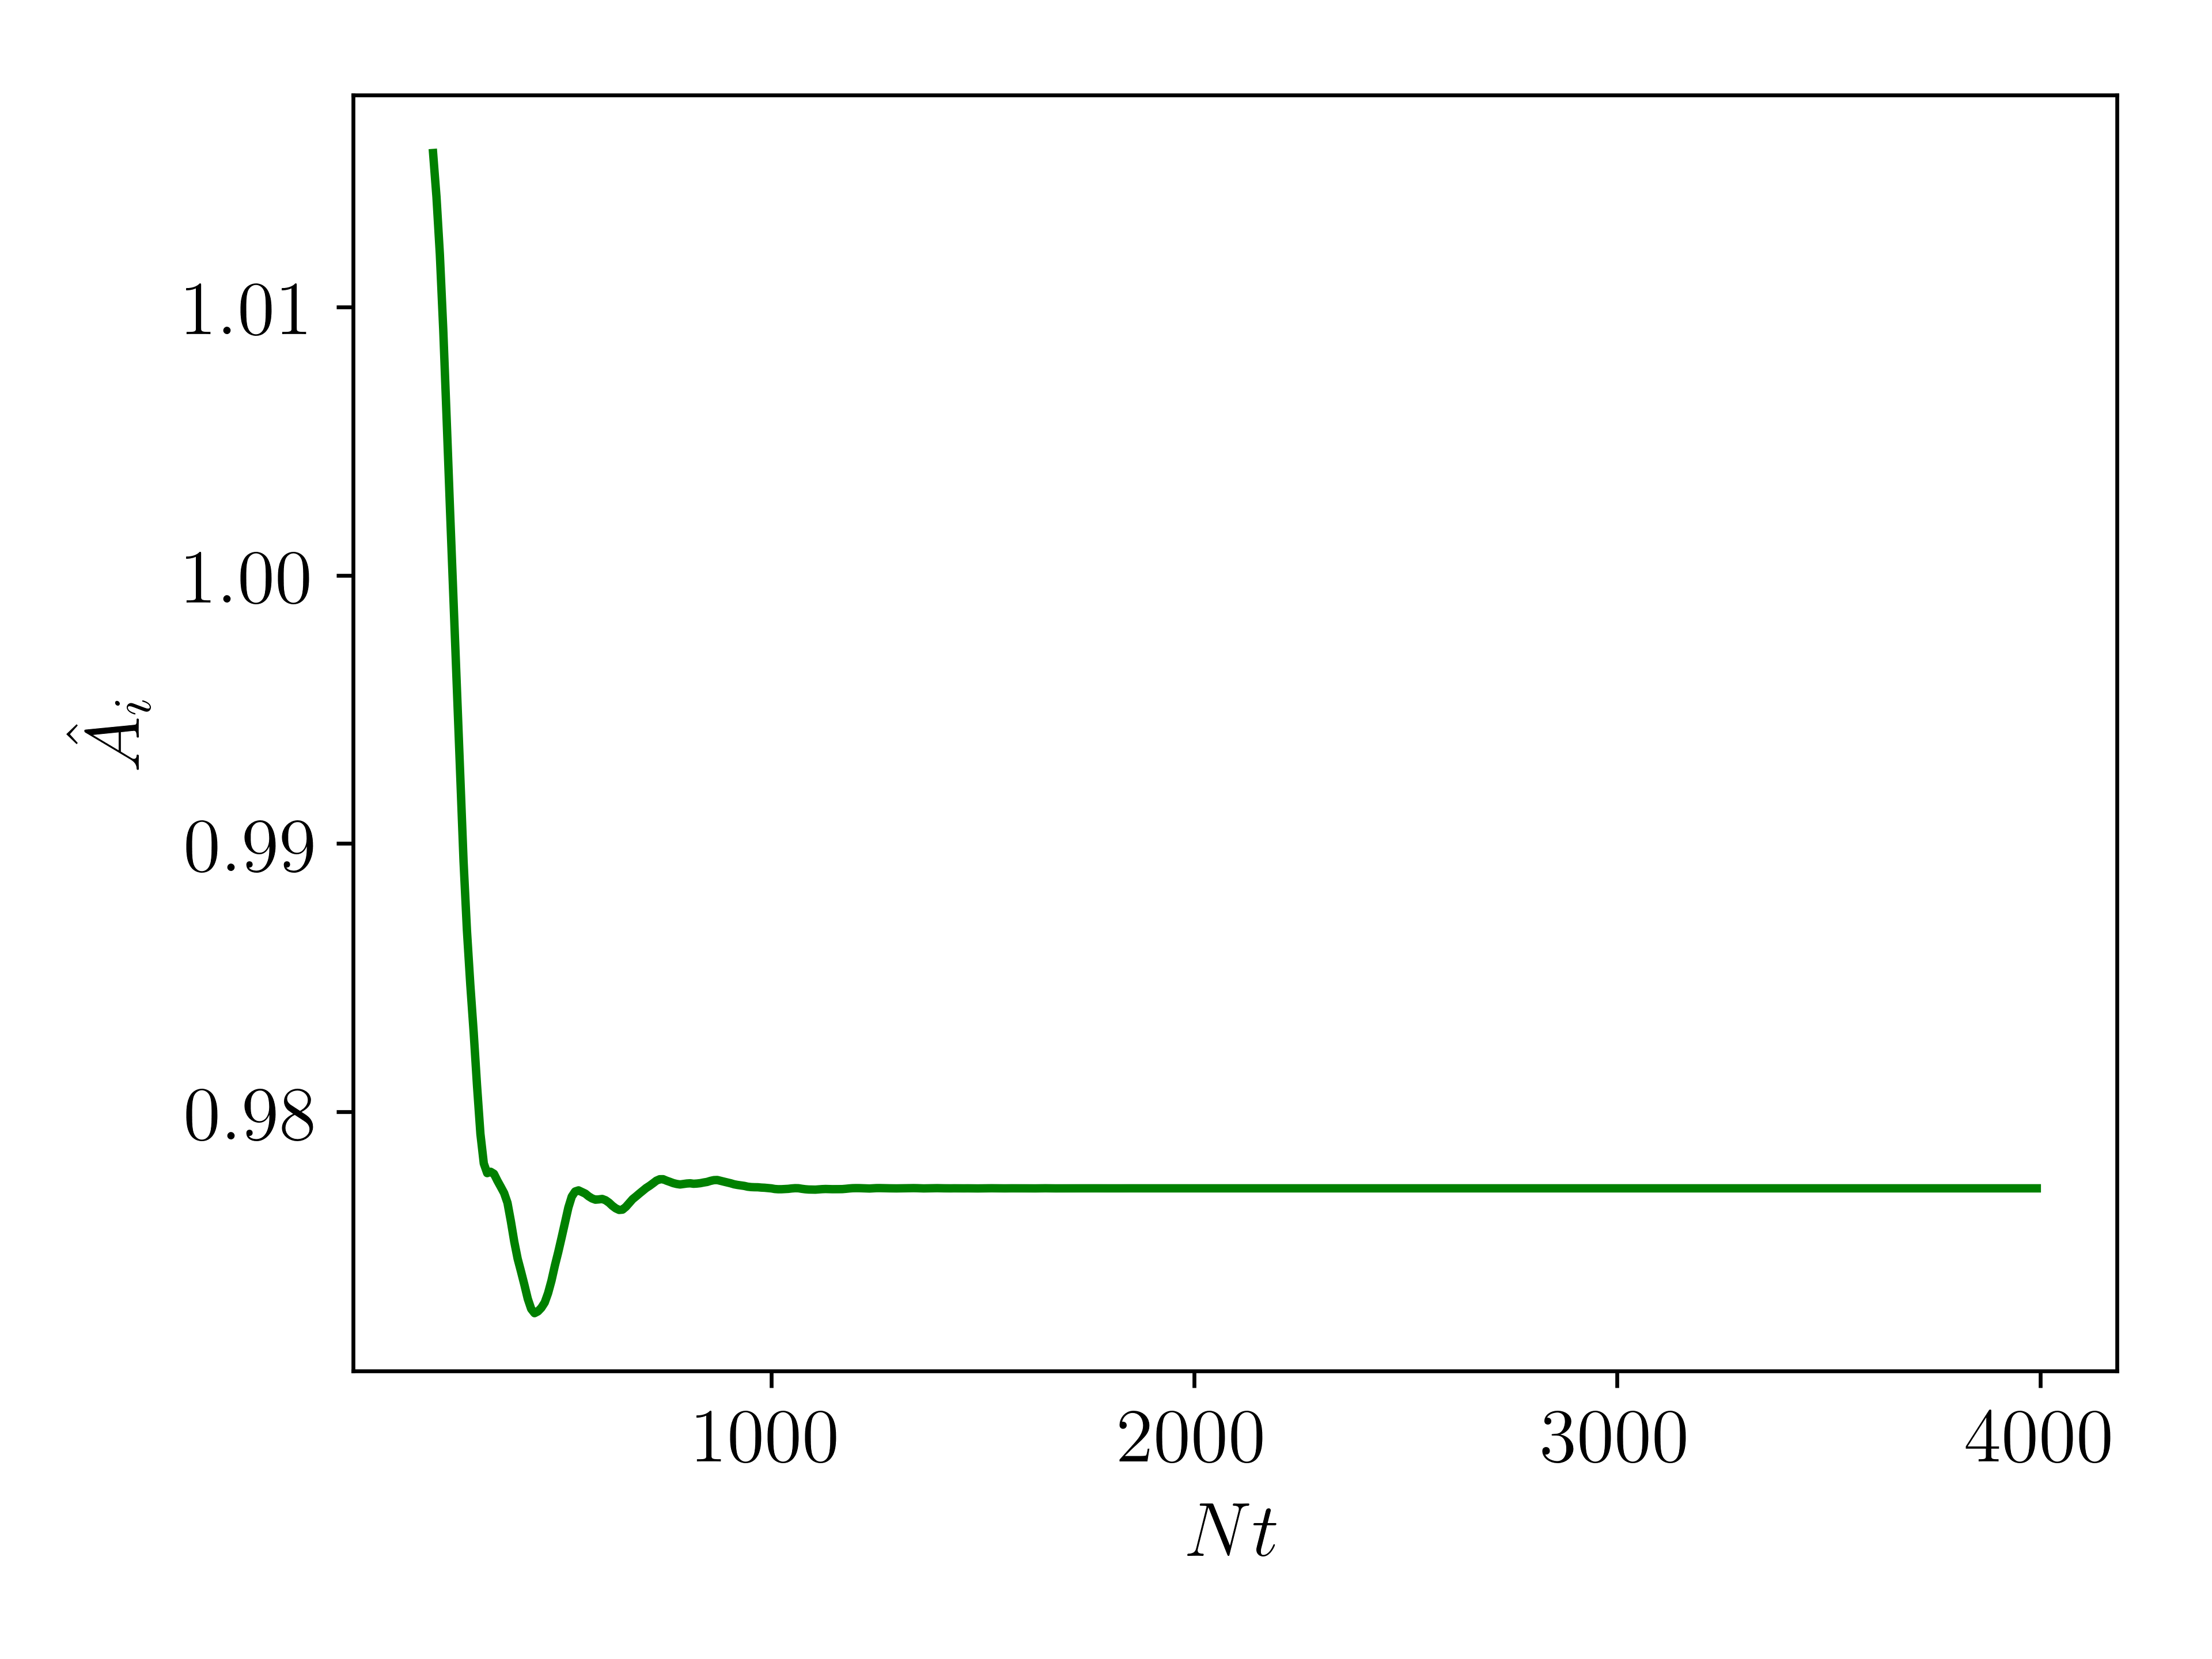
\includegraphics[width=\columnwidth]{plots/lin_amps.png}
    \caption{Amplitude of excited wave over time in weak forcing simulation,
    computed using \autoref{eq:ahat_def}. $A_i(t) = 1$ corresponds to
    perfect agreement with the analytical estimate. After an initial transient
    phase, we observe $A_i(t)$ asymptotes to $\approx 1$, implying continuous
    excitation of identical IGW with the expected amplitude. The small
    suppression may be due to timestepping errors, as a relatively large fixed
    step size $\Delta t = 0.1/N$ was used for this
    simulation.}\label{fig:lin_amps}
\end{figure}

The analytical theory also predicts that the horizontal momentmum flux $F(z, t)$
should be independent of $z$ between the forcing zone where it is generated and
the damping zone where it is dissipated (\autoref{eq:F_def}). We make may a
slightly more accurate estimate of the flux carried in the IGW by directly
substituting $\bm{u}_{al}$ into \autoref{eq:F_def}. Calling this estimate
\begin{equation}
    F_{al}(z) \equiv \ev{\overline{\rho} u_{al,x}u_{al,z}}_x
\end{equation}
we may then measure the agreement of our simulation with analytical expectation
by computing $F$ from the simulation via \autoref{eq:F_def}. Where nonlinear
effects are unimportant, we expect $F(z, t) = F_{al}(z)$.
\autoref{fig:lin_fluxes} shows that $F \approx F_{al}$ between $z_0$ and $z_T$,
as expected.
\begin{figure}
    \centering
    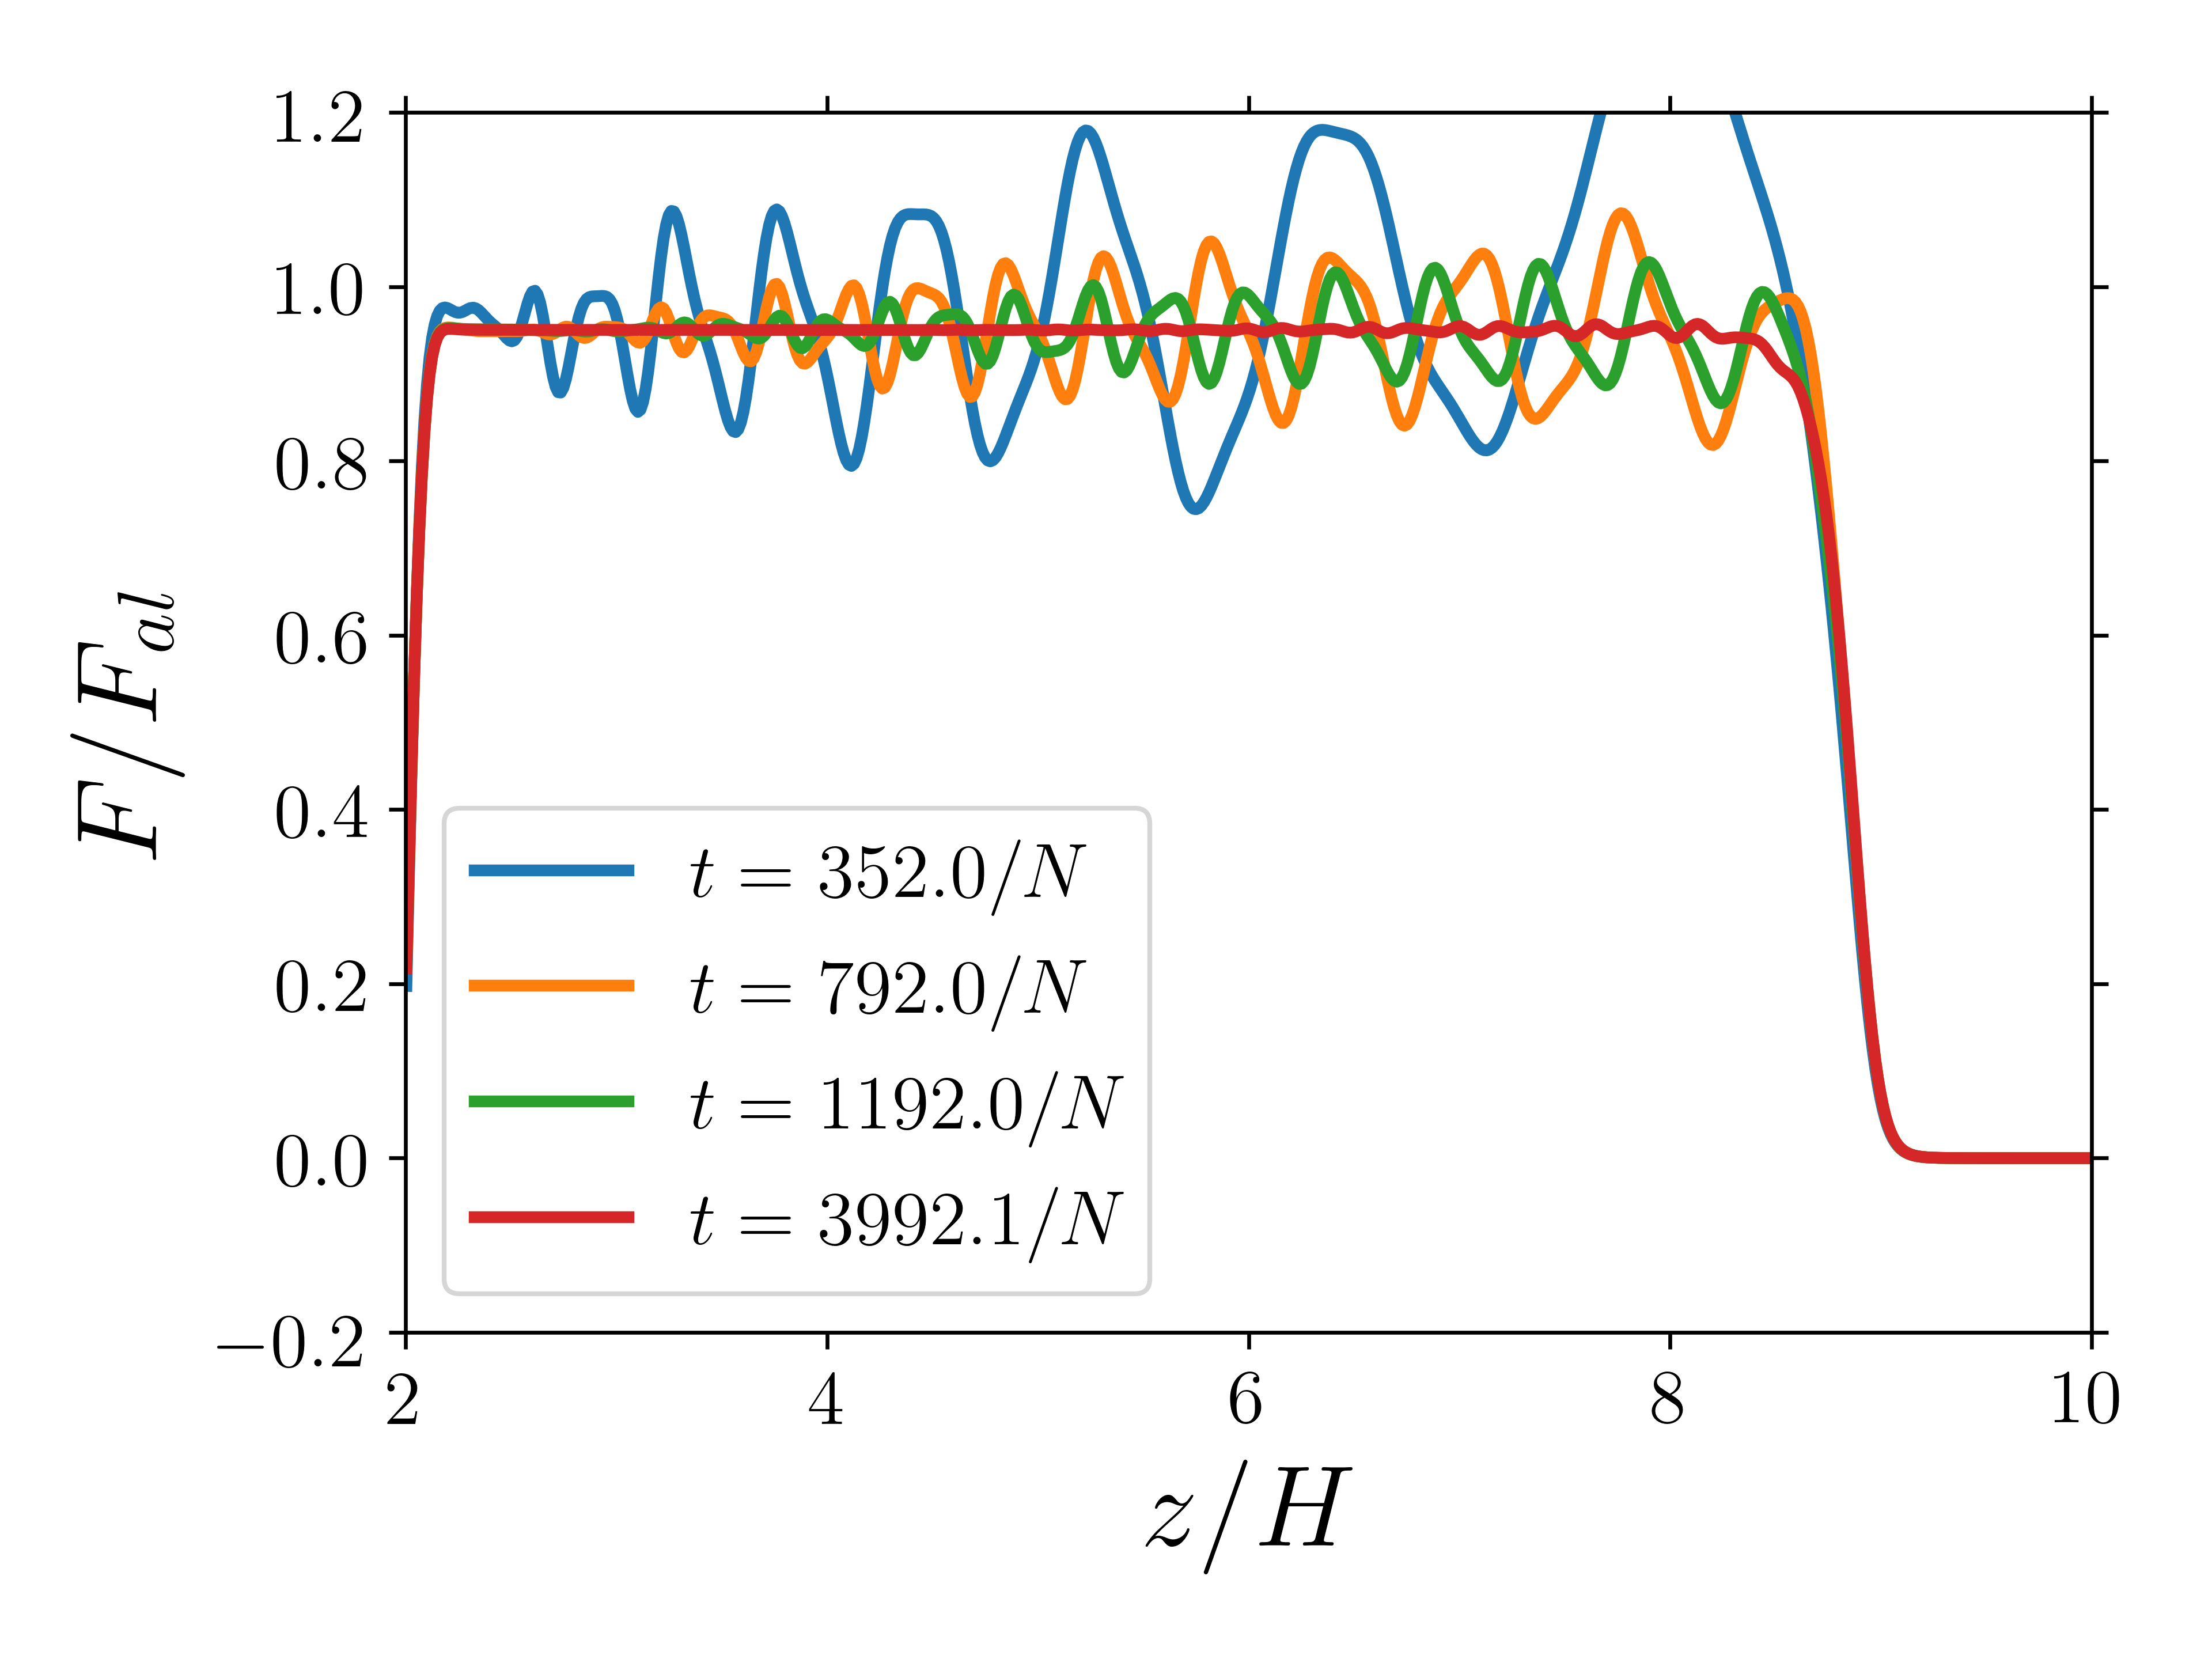
\includegraphics[width=\columnwidth]{plots/lin_fluxes.png}
    \caption{$F/F_{al}$ as a function of $z$ at select times $t$. As
    initial transients die out, $F / F_{al} = 1$ to very good agreement above
    the forcing zone $z > z_0 = 2H$ and below the damping zone $z \lesssim z_T =
    9.5H$. The flux excited in the forcing zone is transported without loss to
    the top of the domain, where it is dissipated by the damping layer (see
    \autoref{ss:damping}) without reflection.}\label{fig:lin_fluxes}
\end{figure}

\section{Numerical Simulations of Wave Breaking}\label{s:sim}

% times on fluxes.png are 054, 086, 153, 451

To perform simulations of wave breaking phenomena, we use the same values as
described in \autoref{s:numerics} except for $C$ and $\nu$. In particular, we
choose $C$ such that $\at{\xi_z k_z}_{z_0} = 0.1$ in the forcing zone. The
linear solution predicts $\xi_z k_z \sim 4.25$ at the upper damping zone $z_T$.
$\mathrm{Re}$ was chosen to be as large as possible across the various
resolutions. A table of our simulations can be found in \autoref{tab:params}.
\begin{table}
    \centering
    \begin{tabular}{l c c c}
        Resolution & $\mathrm{Re}$\\\bottomrule
        $1024 \times 4096$ & $2048$\\
        $768 \times 3072$ & $1024$\\
        $512 \times 2048$ & $512$\\
        $256 \times 1024$ & $341$\\
        $256 \times 1024$ & $205$\\
        $256 \times 1024$ & $146$\\
    \end{tabular}
    \caption{Table of simulation resolutions with wave
    breaking.}\label{tab:params}
\end{table}

\subsection{Numerical Simulation Results}\label{ss:nl_ns}

A full video of our simulation with $N_x = 768$, $N_z = 3072$, $\mathrm{Re} =
1024$ is available
online\footnote{http://www.princeton.edu/~lecoanet/data/breaking\_wave.mov}. We
take this to be our fiducial simulation for the remainder of this paper, though
other simulations show qualitatively similar behavior.

% convert yubo_000054.png -crop 2000x2000+150+250 out.png
In \autoref{fig:snapshots}, we present snapshots of $u_x$ and $\Upsilon$ at
various interesting phases of the simulation. The flow evolves through distinct
stages:
\begin{enumerate}
    \item At early times (top left panel), the flow resembles a linear IGW lower
        in the simulation domain but breaks down into smaller-scale features at
        higher $z$. Some characteristic swirling motion can be seen in the
        advected scalar $\Upsilon$, indicating Kelvin-Helmholtz instabilities.

    \item At a slightly later time (top right panel), the mean flow in
        $u_x$ has become much more prominent and the critical layer $z_c$ has
        become much more definite. Small-scale fluctuations are still present in
        $u_z$ but at smaller amplitudes due to being in a denser region of the
        fluid.

    \item In the bottom left panel, the critical layer transition is now
        extremely sharp, and small swirls of limited vertical extent at the
        location of the critical layer in $u_z$ suggest that the
        Kelvin-Helmholtz instability is responsible for regulating the minimum
        width of this transition. This is supported by the conclusions in
        \autoref{s:khi}.

    \item  The end of the simulation shows very few significant qualitative
        differences from the previous snapshot, suggesting that the latter half
        of our simulation is temporally converged.
\end{enumerate}

\begin{figure*}
    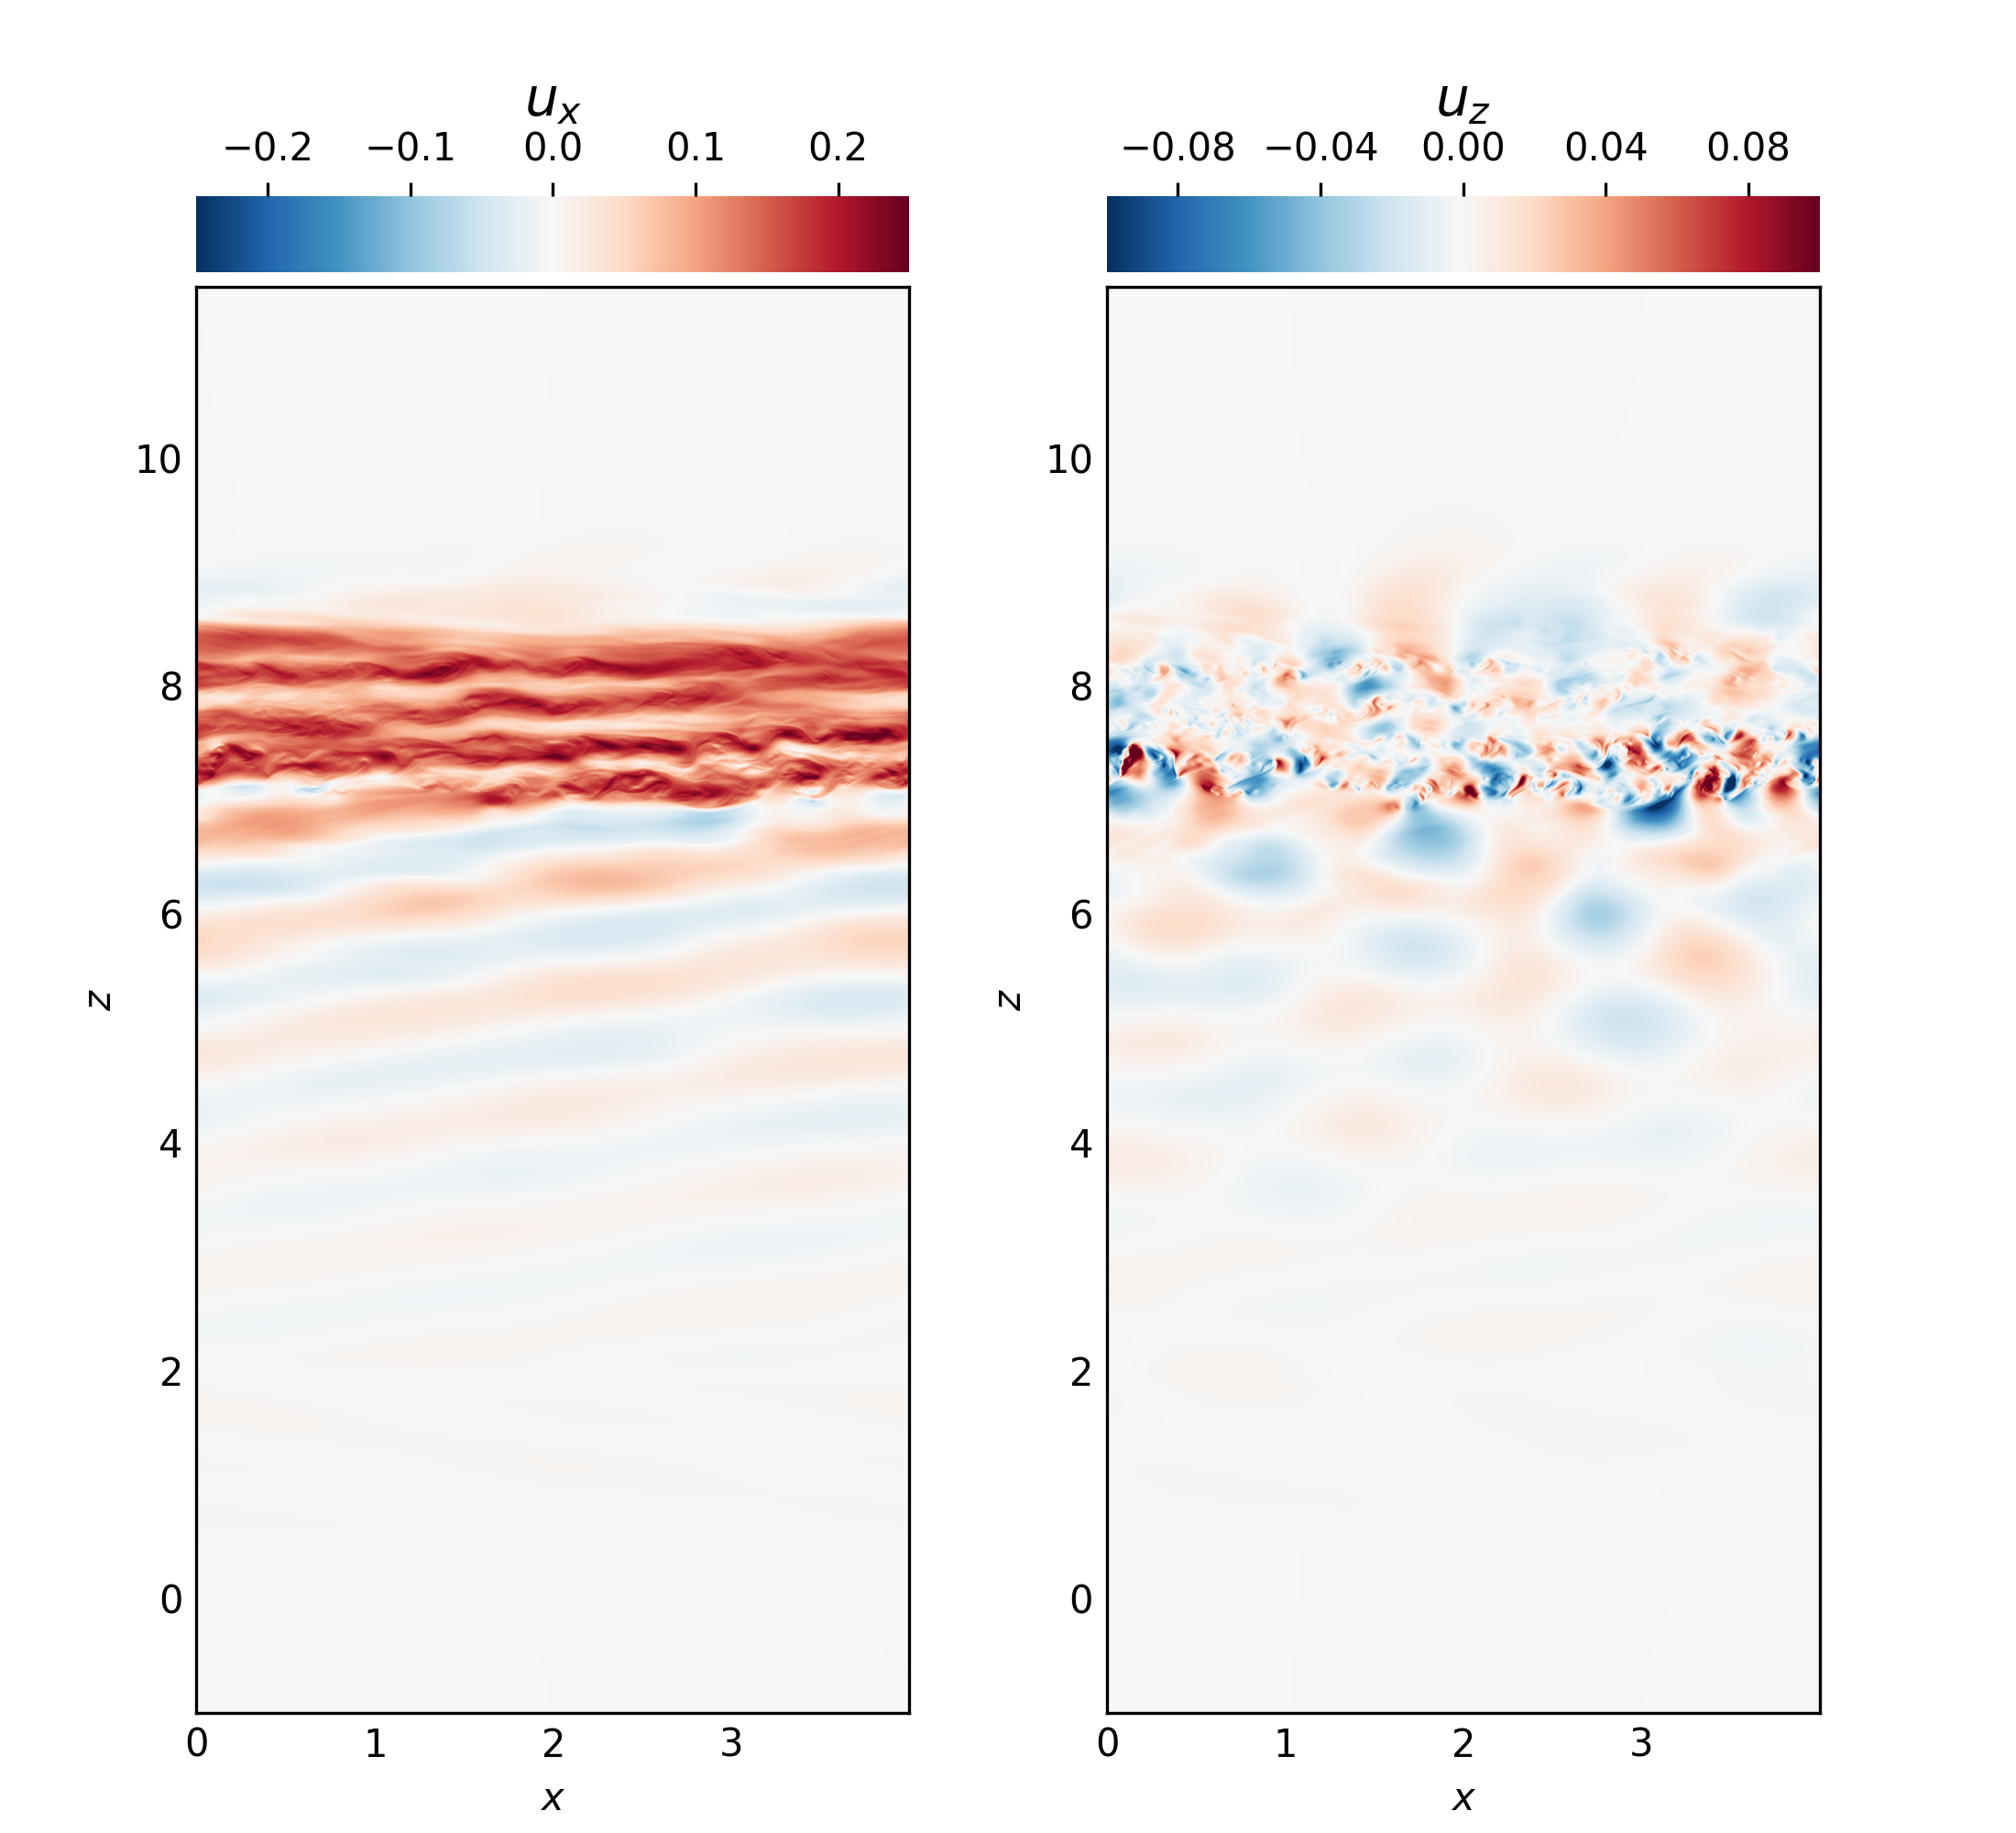
\includegraphics[width=0.45\textwidth]{plots/yubo_000054.png}\hfil
    %
    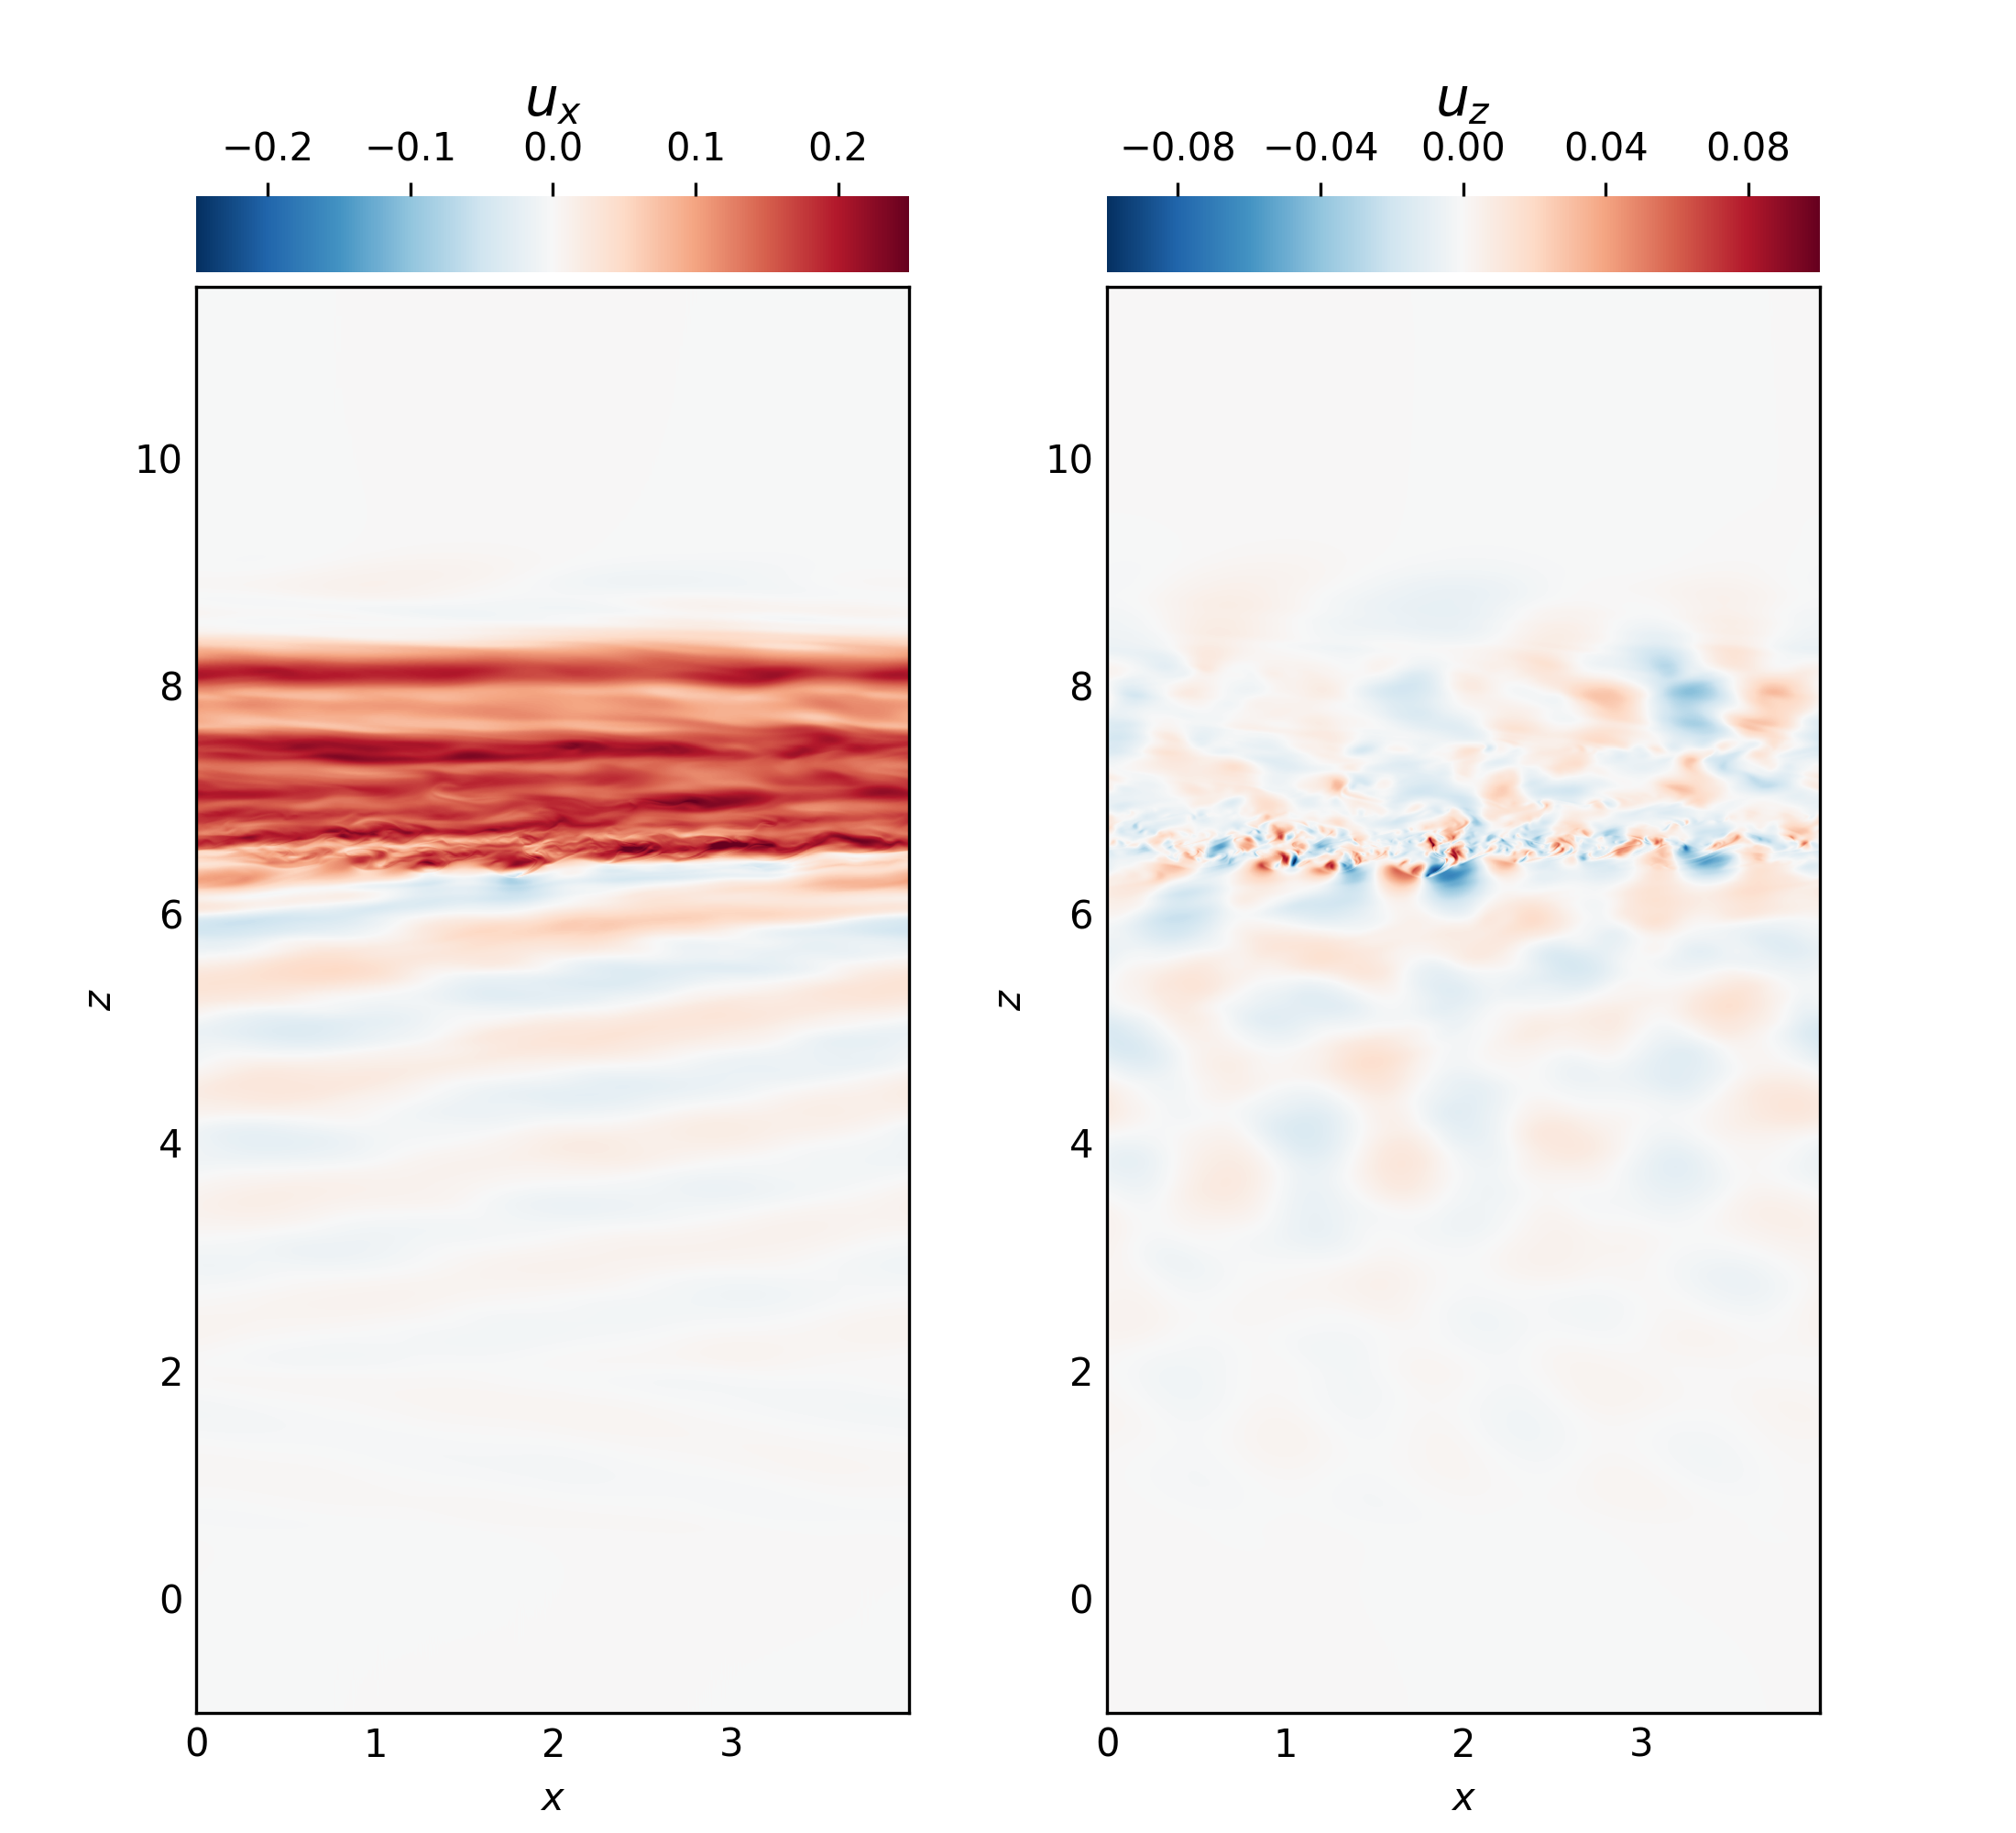
\includegraphics[width=0.45\textwidth]{plots/yubo_000086.png}

    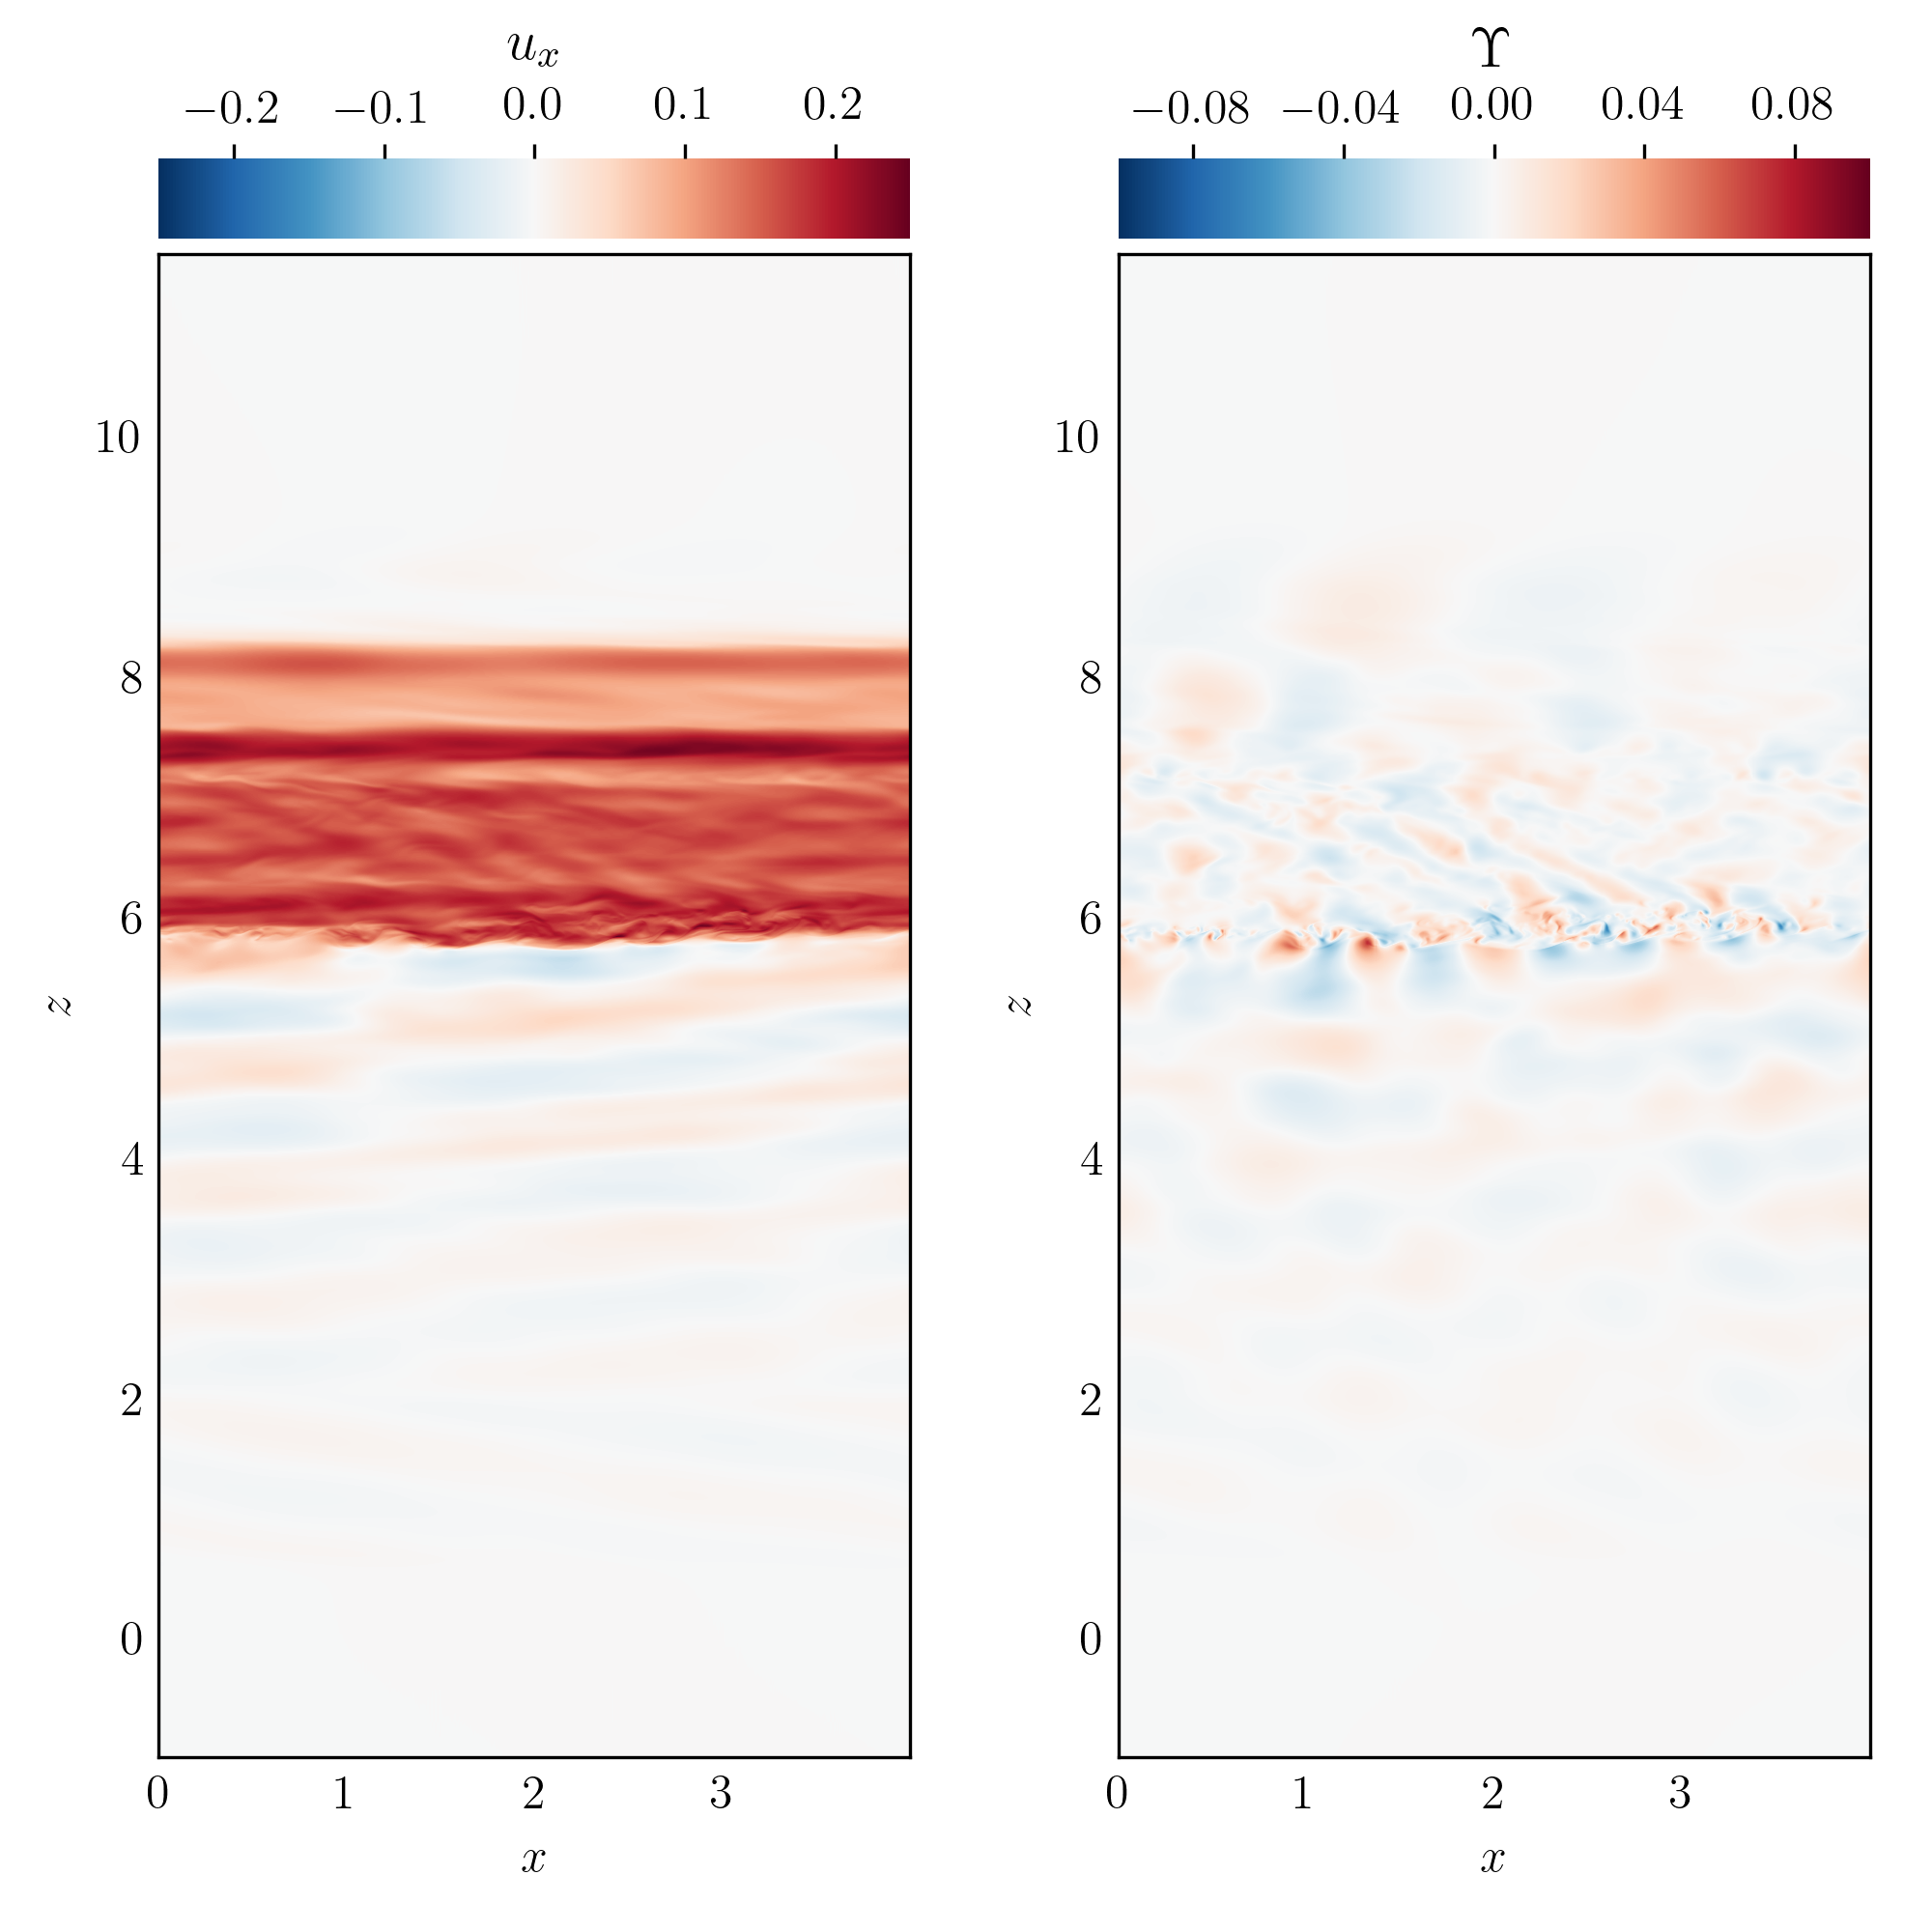
\includegraphics[width=0.45\textwidth]{plots/yubo_000153.png}\hfil
    %
    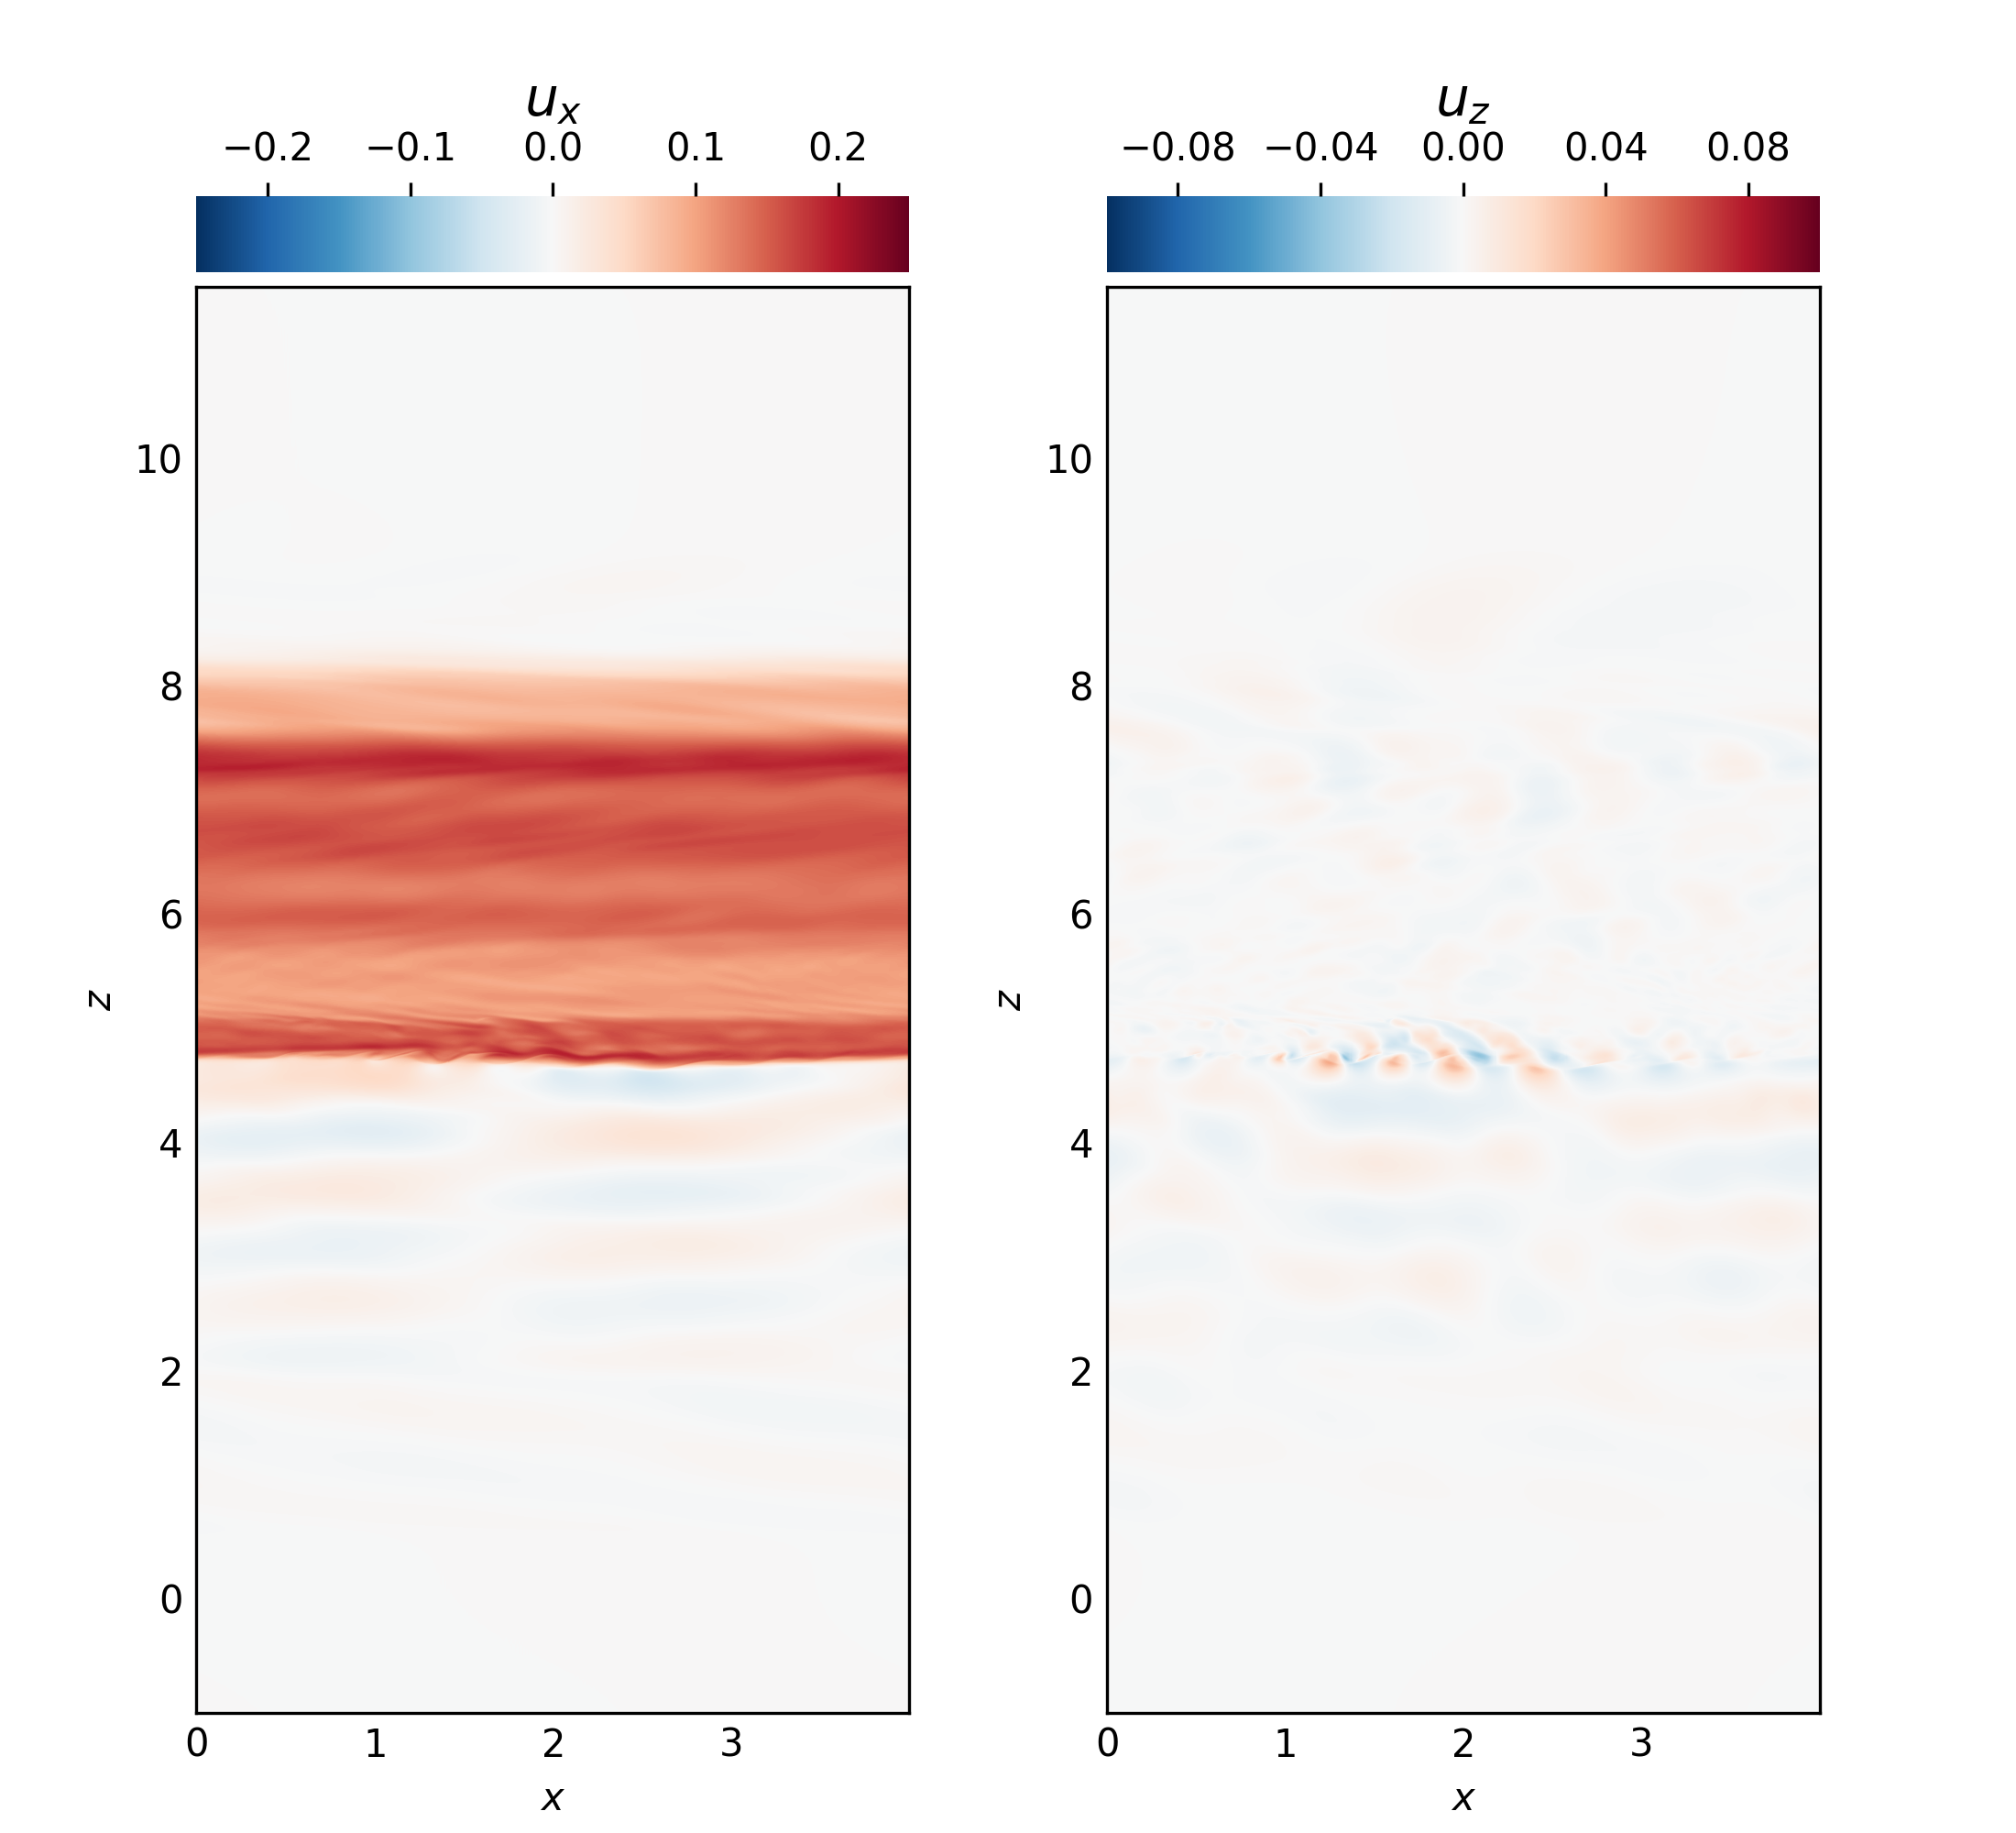
\includegraphics[width=0.45\textwidth]{plots/yubo_000451.png}
    \caption{Snapshots of $u_x, u_z$ in the fiducial simulation illustrating
    distinct phases of the evolution of the flow. Note that $\overline{U}_c
    \approx 0.16HN$ for the parameters used. The four times depicted are $t =
    413.4/N$ (top left), $t = 658.5/N$ (top right), $t = 1171.4/N$ (bottom
    left), and $t = 3437.8/N$ (bottom right). The four snapshots illustrate (i)
    the initial transient wave breaking phase, (ii) formation of a distinct
    critical layer, (iii) steepening of the critical layer, and (iv) propagation
    of the critical layer respectively.}\label{fig:snapshots}
\end{figure*}

In \autoref{fig:nl_fluxes}, we plot $\overline{U}$ and $F / F_{al}$ as a function
of $z$ at the times depicted in \autoref{fig:snapshots}.
At each time, $\overline{U}$ is close to zero below the critical layer, but then
sharply increases to $\overline{U}_c$ at the critical layer. Above the critical
layer, $\overline{U}$ varies slightly due to momentum transport within the
spun-up layer. This is in agreement with the predictions
of \autoref{ss:crit_layer}.

Similarly, $F \lesssim F_{al}$ below the critical layer, and then decreases to
about zero above the critical layer. However, two notable deviations can be
observed: (i) the incident flux on the critical layer seems to fluctuate
somewhat temporally, and (ii) there seems to be a small negative flux above the
critical layer at later times. These are addressed in the following subsection.
\begin{figure}
    \centering
    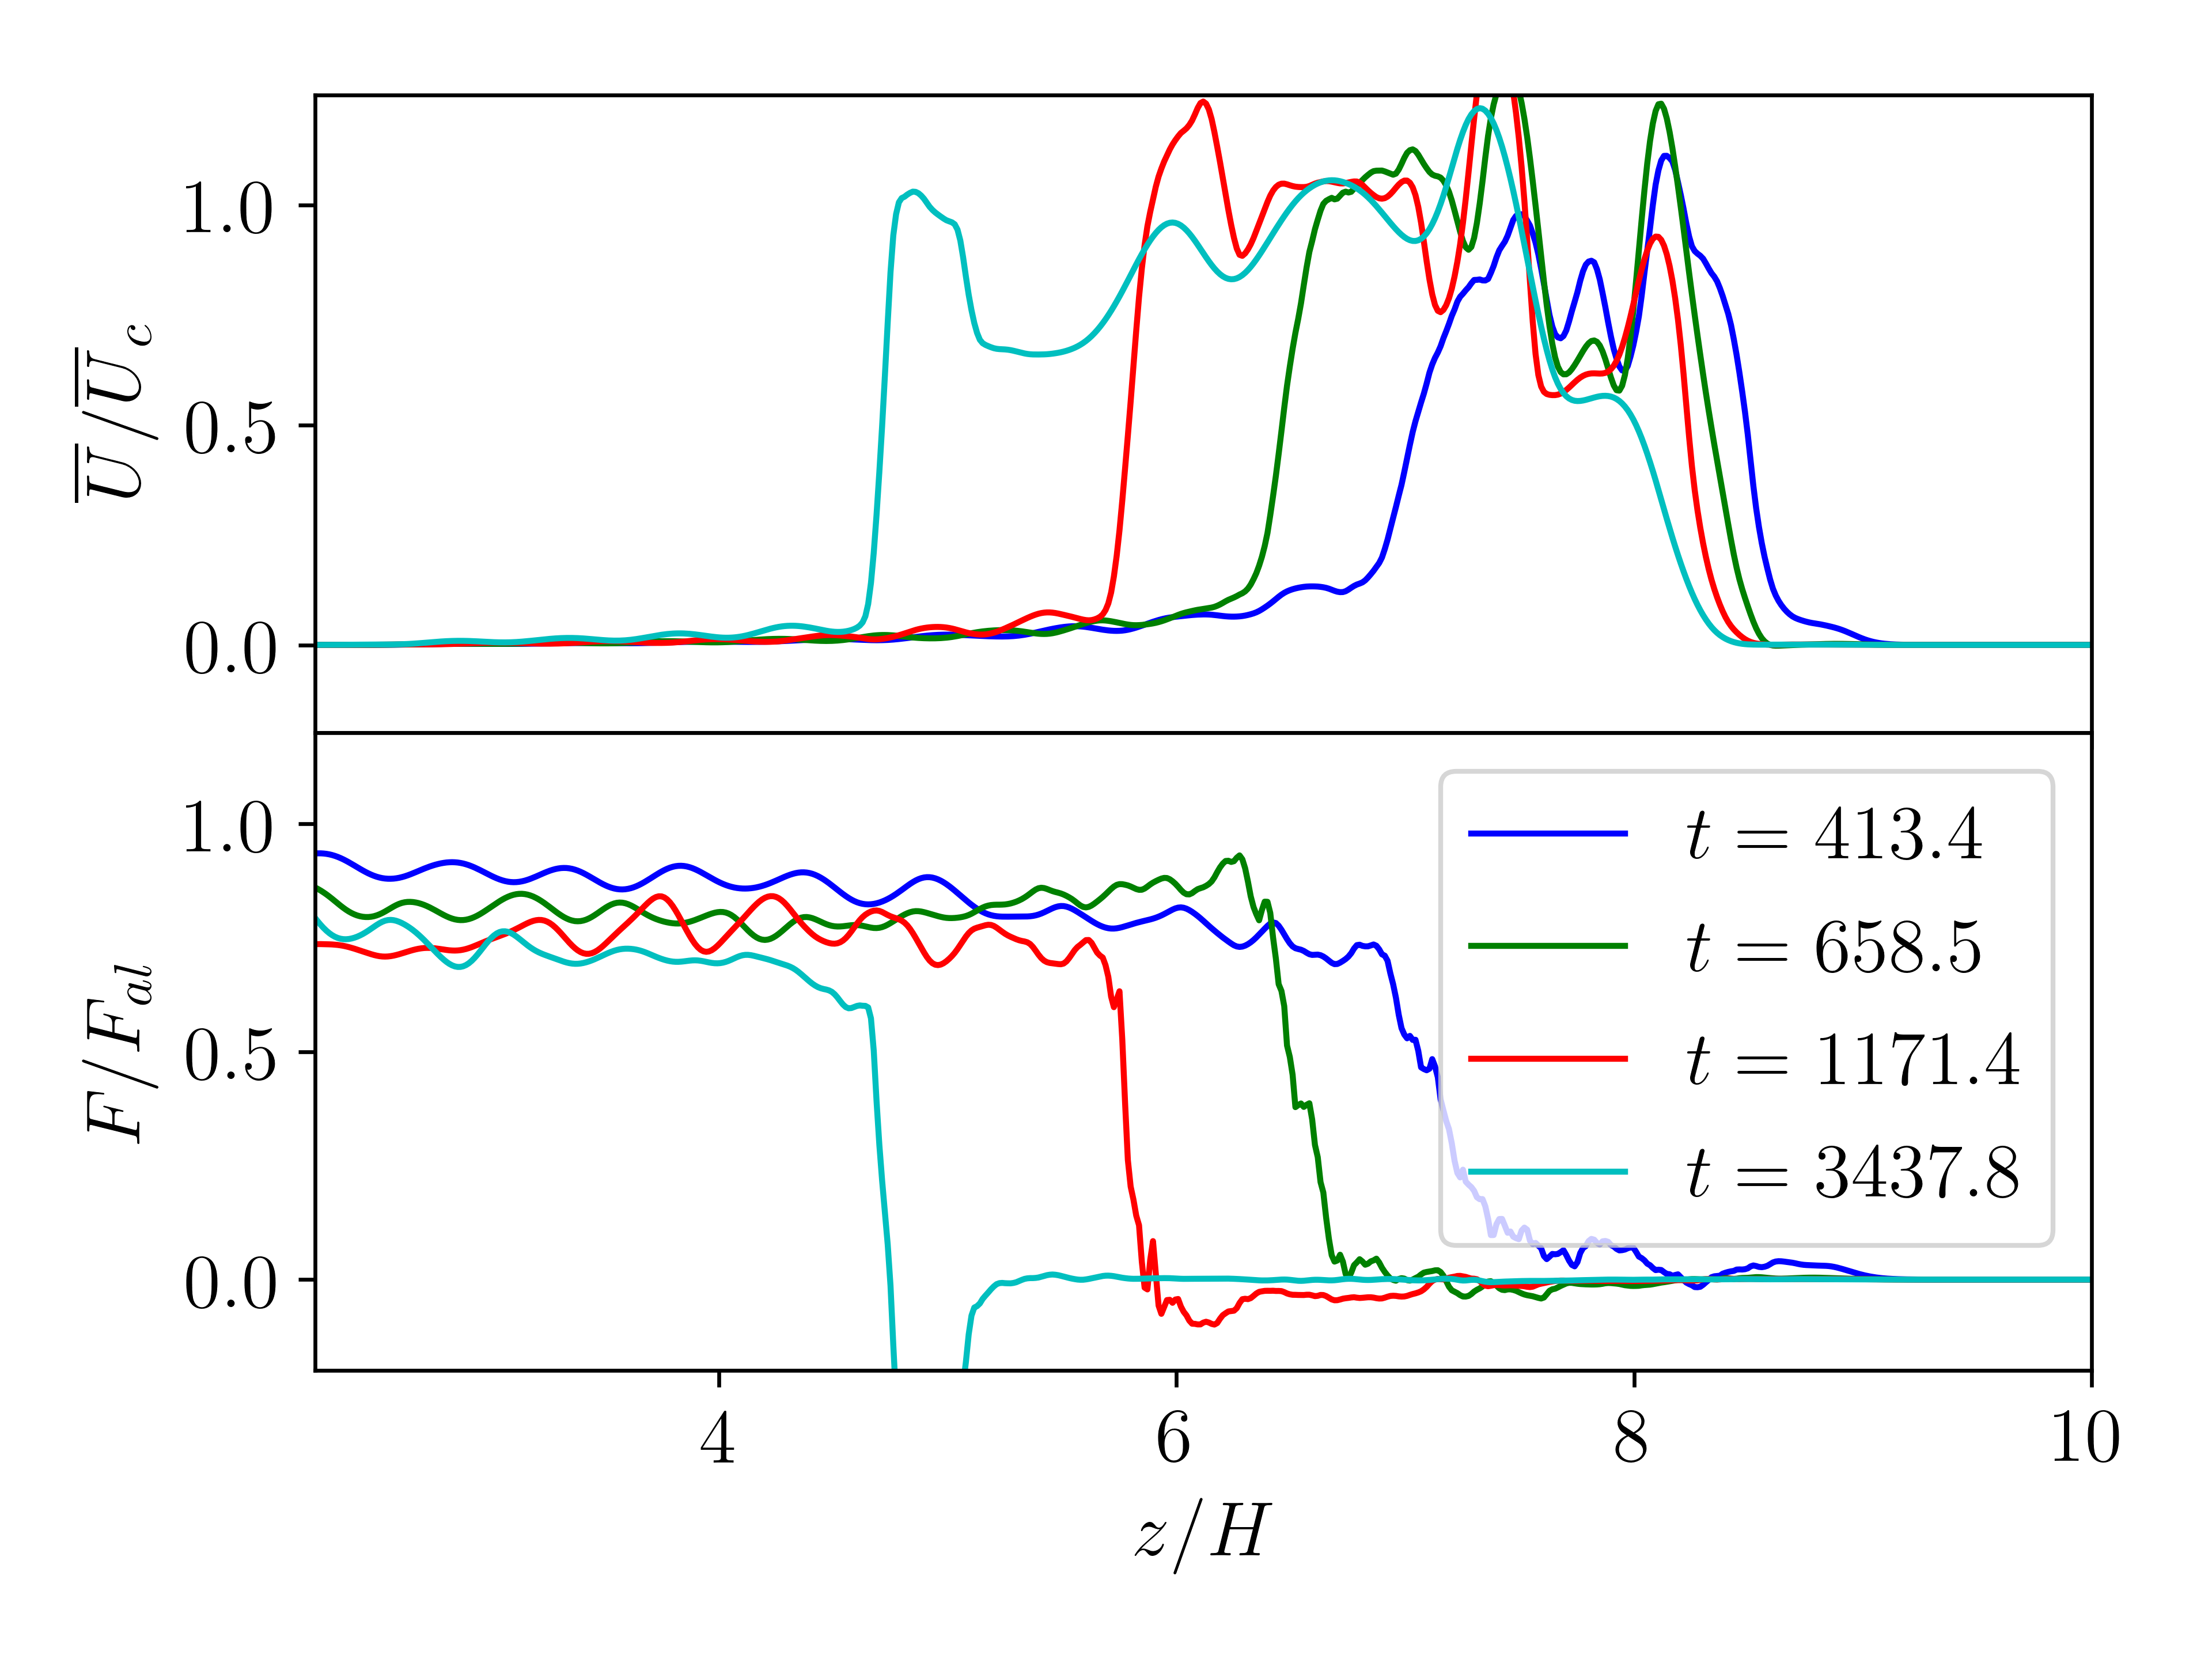
\includegraphics[width=\columnwidth]{plots/nl_fluxes.png}
    \caption{Plot of $\overline{U}(z, t)$ and $F(z, t) / F_{al}(z)$ respectively
    at the same times in \autoref{fig:snapshots} over $z$ in our $\mathrm{Re} =
    1024$ simulation. $\overline{U}, F$ follow their definitions in
    \autoref{eq:mean_flow} and \autoref{eq:F_def}. The two distinct zones of
    mean flow separated by a critical layer, the propagation of this critical
    layer towards lower $z$, and the sharp deposition of $F$ at the critical
    layer are evident.}\label{fig:nl_fluxes}
\end{figure}

\subsection{Flux Budget}\label{ss:flux_budget}

The propagation of the critical layer $z_c(t)$ is driven by the absorbed flux at
$z_c$, following \autoref{eq:zc_anal}. When analyzing the simulation, one must
first compute $z_c$ before analyzing the flux budget in its vicinity, but
conceptually $z_c$ is a consequence of flux redistribution at the critical
layer. We proceed in conceptual order and first describe how we analyze the flux
transfer at $z_c$.

In general, the flux budget at the critical layer can be decomposed as
\begin{equation}
    F_i(t) = F_a(t) + F_r(t) + F_s(t),
\end{equation}
where $F_i > 0$ is the incident flux, $F_a > 0$ is the absorbed flux, $F_r > 0$
is the reflected flux, and $F_s < 0$ is some flux above the critical layer,
likely responsible for momentum redistribution within the synchronized outer
zone of the WD\@. Careful accounting of $F_s$ turns out to be important to
obtain the correct critical layer propagation. A more specific physical
interpretation of $F_s$ is unclear; it is somewhat tempting but unfounded to
identify $F_s$ with some transmitted flux.

After measuring $z_c$ at each time (see \autoref{ss:cl_prop}), we can then
determine each of $F_i$, $F_a$, $F_r$, $F_s$ as follows:
\begin{align}
    F_i(t) &= \ev{\rho u_{x} u_{z}}_xA_i^2(t),\\
    F_i(t) - F_r(t) &= \ev{F(z)}_{z \in [z_c - \Delta z - H, z_c - \Delta z]}
        ,\label{eq:fr_def}\\
    F_s(t) &= \ev{\z{F(z): F(z) < 0}}_{z \in [z_c, z_c + \Delta z]},
        \label{eq:fs_def}\\
    F_a(t) &= F_i - F_r - F_s.\label{eq:fa_def}
\end{align}
Here, $\ev{\dots}_{z \in [z_a, z_b]}$ denotes an average over the interval
$[z_a, z_b]$. Below the critical layer, we average over an interval of length
$\frac{2\pi}{k_{z}}$ a full vertical wavelength. The offset $\Delta z$ is
necessary to make a measurement of the incident flux unaffected by the
turbulence within the critical layer itself. The height of the critical layer is
limited by $\mathrm{Ri} \lesssim 1$ (see \autoref{s:khi}), which bounds its
vertical extent $\sim \frac{1}{k_{z}}$. We empirically found an offset of
$\Delta z = \frac{3}{k_z}$ was necessary to be sufficiently far from strong
fluctuations near the critical layer.

Above the critical layer, we observe that the $F_s$ feature has varying width
(see \autoref{fig:nl_fluxes} again) but contributes significantly to the total
flux budget. We average only where $F < 0$ to be robust to such width
variations, and this was found to be a sufficiently accurate way of measuring
$F_s$.

\subsection{Critical Layer Propagation}\label{ss:cl_prop}

With a careful determination of $F_a$, we can next make predictions for the
propagation of $z_c(t)$ and compare to the observed propagation.
In principle, $z_c$ is the location where the incident flux significantly
attenuates. In the simulations, shear turbulence causes $F$ to have significant
spatial and temporal fluctuations that propagate to large temporal fluctuations
in $z_c(t)$. To minimize these spurious fluctuations, we measure the location of
the critical layer using a spatial average of where flux deposition occurs
\begin{align}
    z_{c, \min}(t) &\equiv \argmin_z \z{z: F(z, t) > 0.3F_{al}},\\
    z_{c, \max}(t) &\equiv \argmax_z \z{z: F(z, t) < 0.3F_{al}},\\
    z_c(t) &\equiv \frac{z_{c, \min}(t) + z_{c, \max}(t)}{2}.\label{eq:zc_def}
\end{align}
Measuring $z_c$ in other ways does not significantly change the results of the
analysis.

Finally, we may plot the measured $z_c$ against two semi-analytic predictors:
(i) integration of \autoref{eq:zc_anal} using the measured $F_a(t)$, and
(ii) substituting the time-averaged $\ev{F_a}_t$ (over the entire length of
the simulation) into \autoref{eq:zc_sol}. Since $z_c(t)$ is both unstable and
less well-defined at early times (when the critical layer is thick and transient
behavior is still strong), we solve \autoref{eq:zc_anal} by integrating
backwards from the end of the simulation, using $z_c(t_f)$ as initial condition.
The resulting predictors are depicted in \autoref{fig:nl_front}. The good
agreement between the evolution of $z_c(t)$ and its estimate via $F_a(t)$ and
\autoref{eq:zc_anal} are noteworthy.

The behavior of the behavior of the fiducial, time-averaged $\ev{F_a}_t =
0.71F_{al}$ predictor provides interesting insights. The general agreement
clearly demonstrates $F_a < F_{al}$ and that momentum flux absorption is
not complete. However, its underprediction of critical layer velocity at early
times contrasts with its overprediction at later times. This suggests that
momentum flux absorption changes significantly over time, in agreement with
detailed analysis in \autoref{ss:reflectivity}.
\begin{figure}
    \centering
    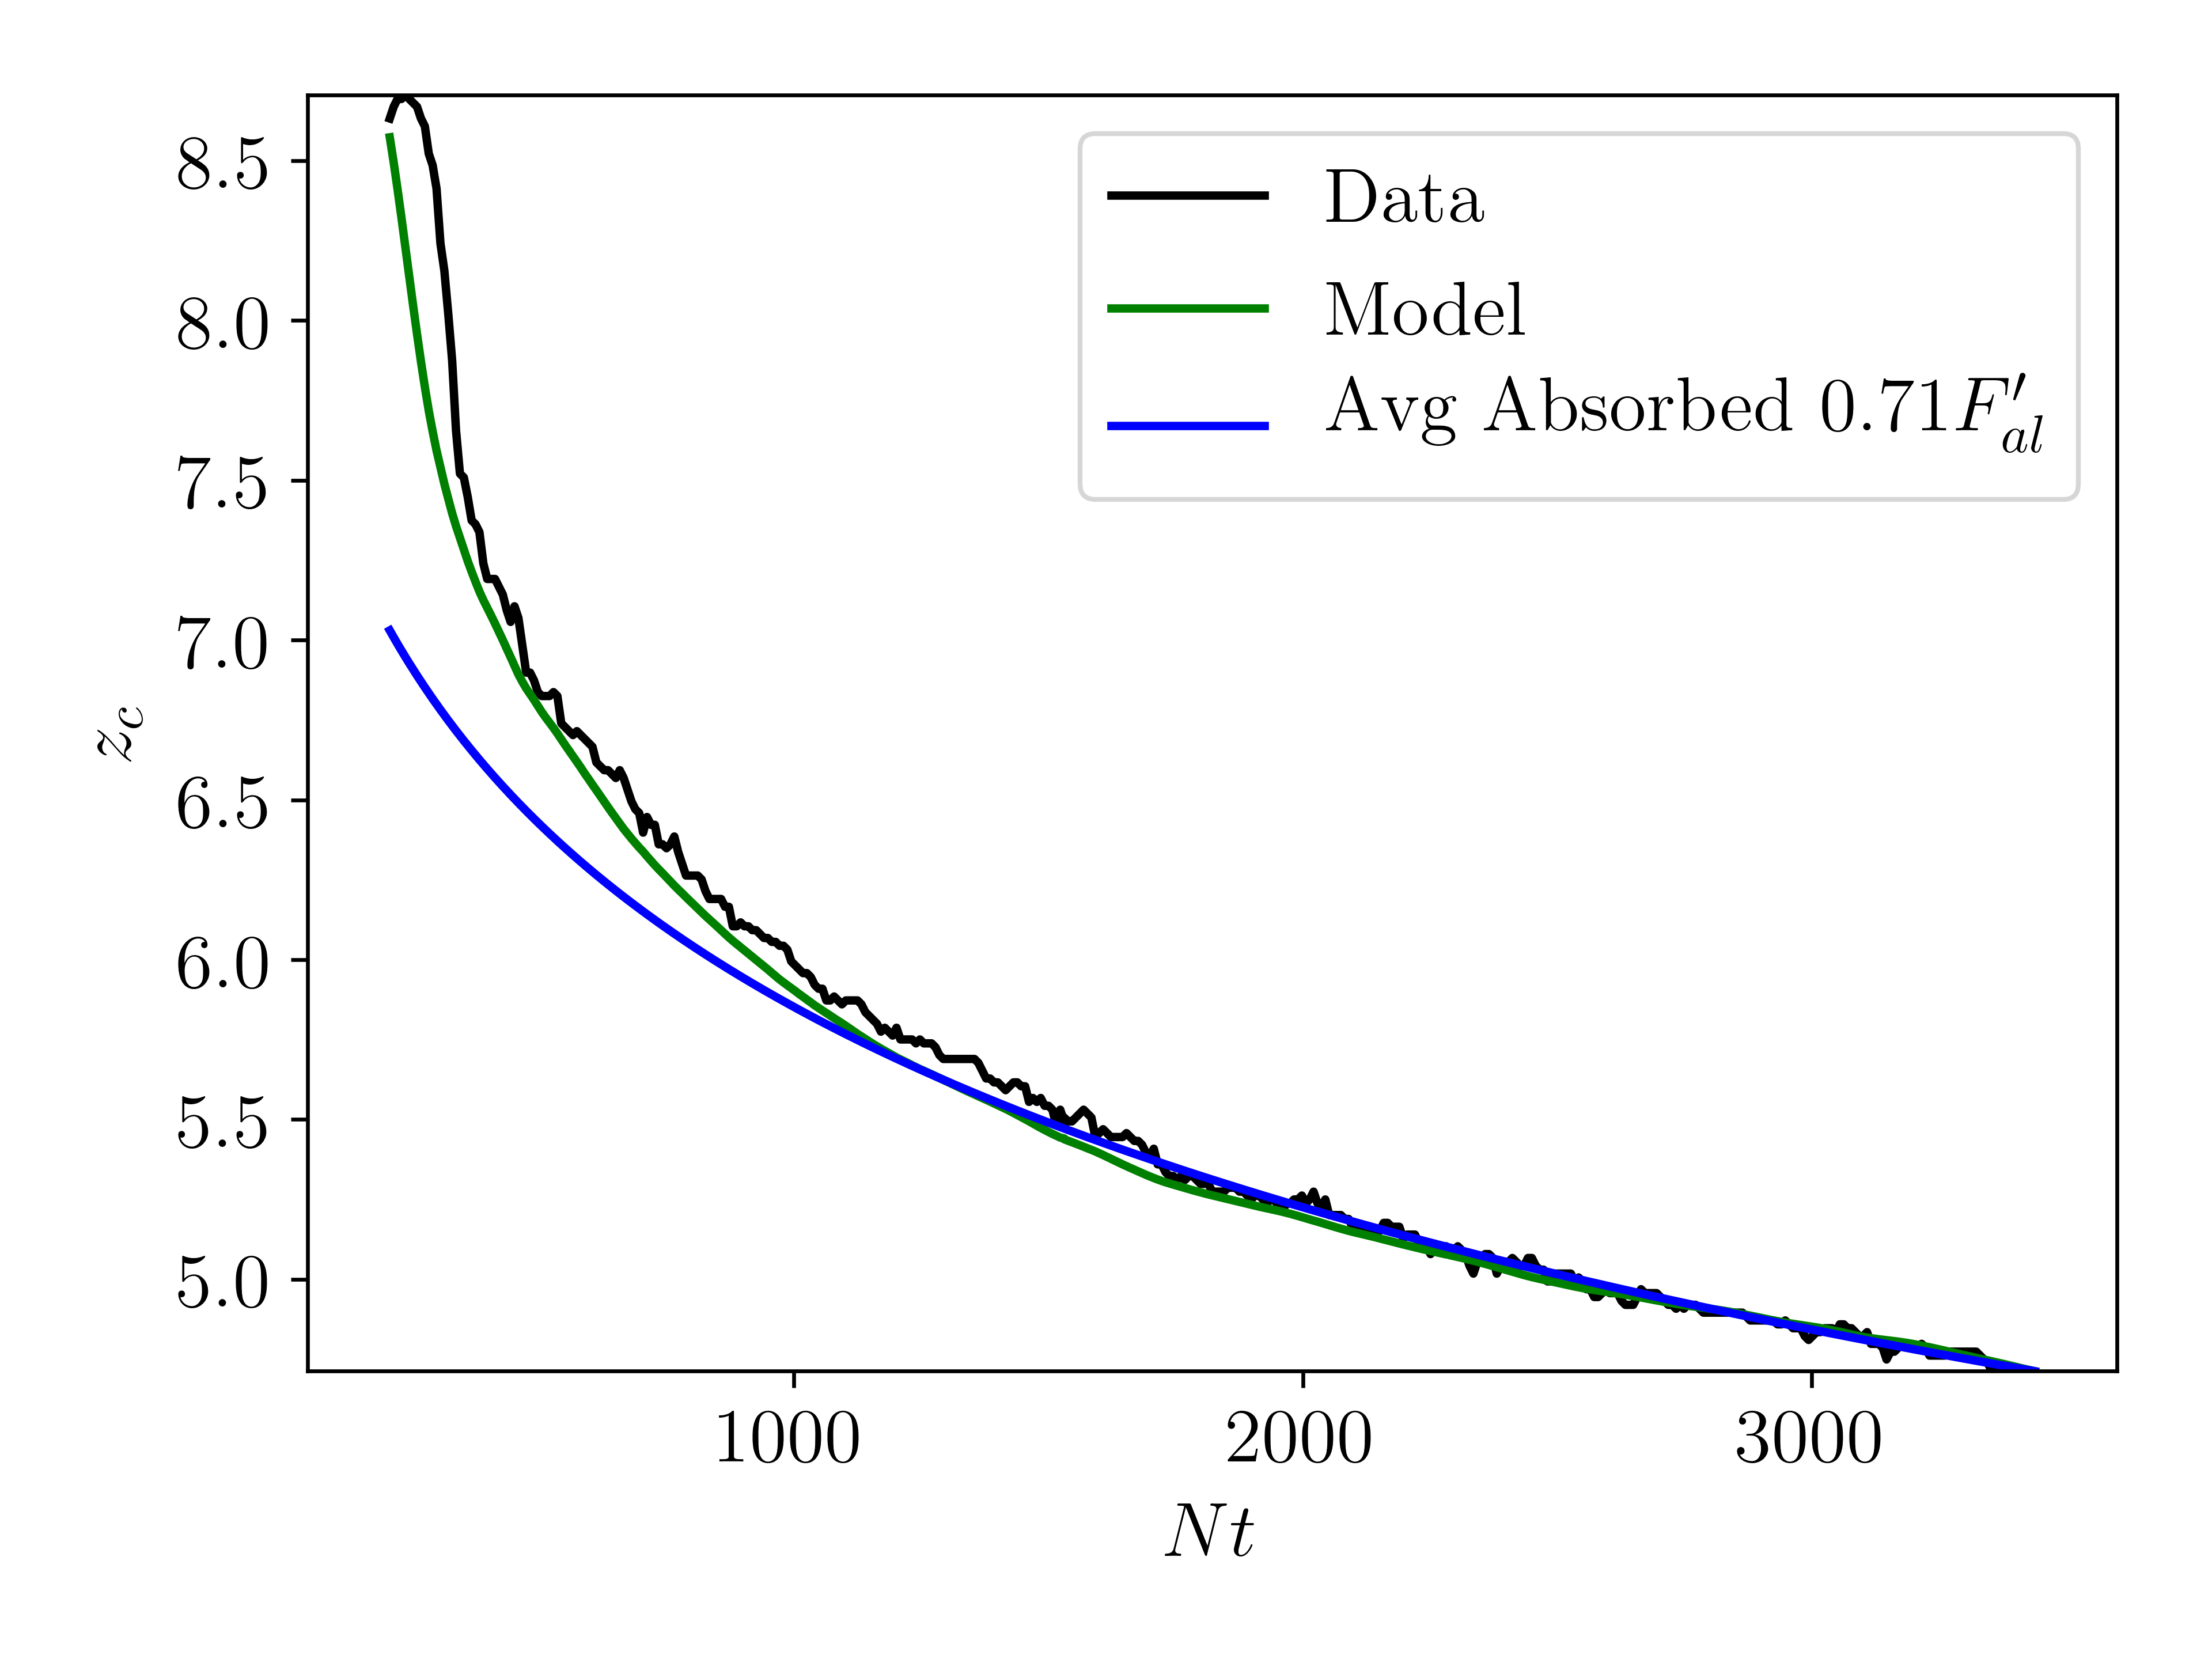
\includegraphics[width=\columnwidth]{plots/nl_front.png}
    \caption{Propagation of the critical layer over time. Shown are (black)
    $z_c(t)$ from simulation data, (green) predictor of $z_c(t)$ using direct
    integration of \autoref{eq:zc_anal} for $F_a(t)$ measured from
    simulation data (described in \autoref{eq:fa_def}) and (blue) direct
    substitution of time-averaged $\ev{F_a(t)}_t$ into
    \autoref{eq:zc_sol}. Predictors use the end of the simulation as initial
    conditions and integrate backwards, as $z_c$ is less well-defined at early
    times. The agreement of the directly-integrated predictor with the data
    shows \autoref{eq:zc_anal} is a good description of the evolution of $z_c$.
    The the poorer but qualitatively correct agreement of the time-averaged
    predictor with the data shows both that $F_a(t) \neq F_{al}$ and that
    $F_a(t)$ likely varies in time.}\label{fig:nl_front}
\end{figure}

\subsection{Non-absorption at Critical Layer}\label{ss:reflectivity}

To further understand the behavior at the critical layer, we compare two
reflective behaviors observed in the simulation: (i), the presence of a
reflected wave with wave vector $\bm{k}_r = k_{x}\uv{x} - k_{z}\uv{z}$, and (ii)
$F_r$. The reflected wave amplitude and reflected flux need not agree exactly if
some reflected flux is in higher-order modes, which is indeed the case in our
simulations. Both are of physical interest, however: the reflected wave
amplitude may be of physical interest in setting up standing modes in a
realistic star, while the flux transfer properties is important for accurately
tracking angular momentum transfer during synchronization.

To measure the reflected wave amplitude $A_r(t)$, we use \autoref{eq:ahat_def}
with $\bm{u}_{al}$ computed with $\bm{k}_r$ with one key change: since the phase
of the reflected wave is unknown, unlike that of the incident wave, we fit for
an arbitrary horizontal offset $\delta x(t)$ at each time $t$ (not constrained
to be on-grid), picking $\delta x$ that maximizes $A_r$. To be explicit, we
compute
\begin{equation}
    A_r(t) = \max_{\delta x}\frac{\int\limits_{z_b}^{z_t}\int\limits_0^{L_x}
        \overline{\rho}\p{\bm{u} \cdot \at{\bm{u}_{al,
        \bm{k}_r}}_{x = x + \delta x}}\;\mathrm{d}x\mathrm{d}z}
        {\int\limits_{z_b}^{z_t}\int\limits_0^{L_x}
        \overline{\rho}\abs{\bm{u}_{al}}^2\;\mathrm{d}x\mathrm{d}z}
        \label{eq:ar_def}
\end{equation}
In our simulations, the phase offset $\phi_r(t) \equiv k_x \delta x(t) $ behaves
in agreement with reflection off a moving boundary at $z_c$, well approximated
by $\abs{\pd{\phi_r}{t}} \approx 2\abs{\pd{(k_{z}z_c)}{t}}$.

Since reflectivity depends sensitively on accurate measurements of $A_i,
A_r$, we remark \autoref{eq:ahat_def} and \autoref{eq:ar_def} ensure
orthogonality between $k_{x}\uv{x} \pm k_{z}\uv{z}$ modes. The integral for
$A_r$ is also performed over $z \in [z_0 + 3\sigma, z_0 + 3\sigma + H]$. Since
$A_i(t), A_r(t)$ vary somewhat strongly over time, we perform time averaging
over interval approximately $8\pi/\omega$, denoted by angle brackets. We can
then define the amplitude reflectivity
\begin{equation}
    \mathcal{R}_A(t) \equiv \frac{\ev{A_r}(t)}{\ev{A_i}(t)}
        .\label{eq:Ra_def}
\end{equation}
% 7/N per timestep, 13 timestep smoothing kernel, 24/N period

To compare to the behavior of the flux at the critical layer, we compare
$\mathcal{R}_A^2(t)$ to the ratios of $F_r$ and $F_s$ to $F_i$. We define
shorthand
\begin{align}
    \hat{F}_r &\equiv \frac{\ev{F_r}(t)}{\ev{F_i}(t)},
        \label{eq:srefl_def1}\\
    \hat{F}_s &\equiv -\frac{\ev{F_s}(t)}{\ev{F_i}(t)}.
        \label{eq:srefl_def}
\end{align}
\autoref{fig:nl_f_amps} demonstrates the relations between these quantities. All
of these quantities vary significantly temporally but their mean values appear
to converge towards the end of the simulation. A significant fluctuation in
$A_i(t)$ is observed. We were unable to identify the cause of this unintended
fluctuation, but it doees not affect $\mathcal{R}_A$ thanks to the time
averaging used.
\begin{figure}
    \centering
    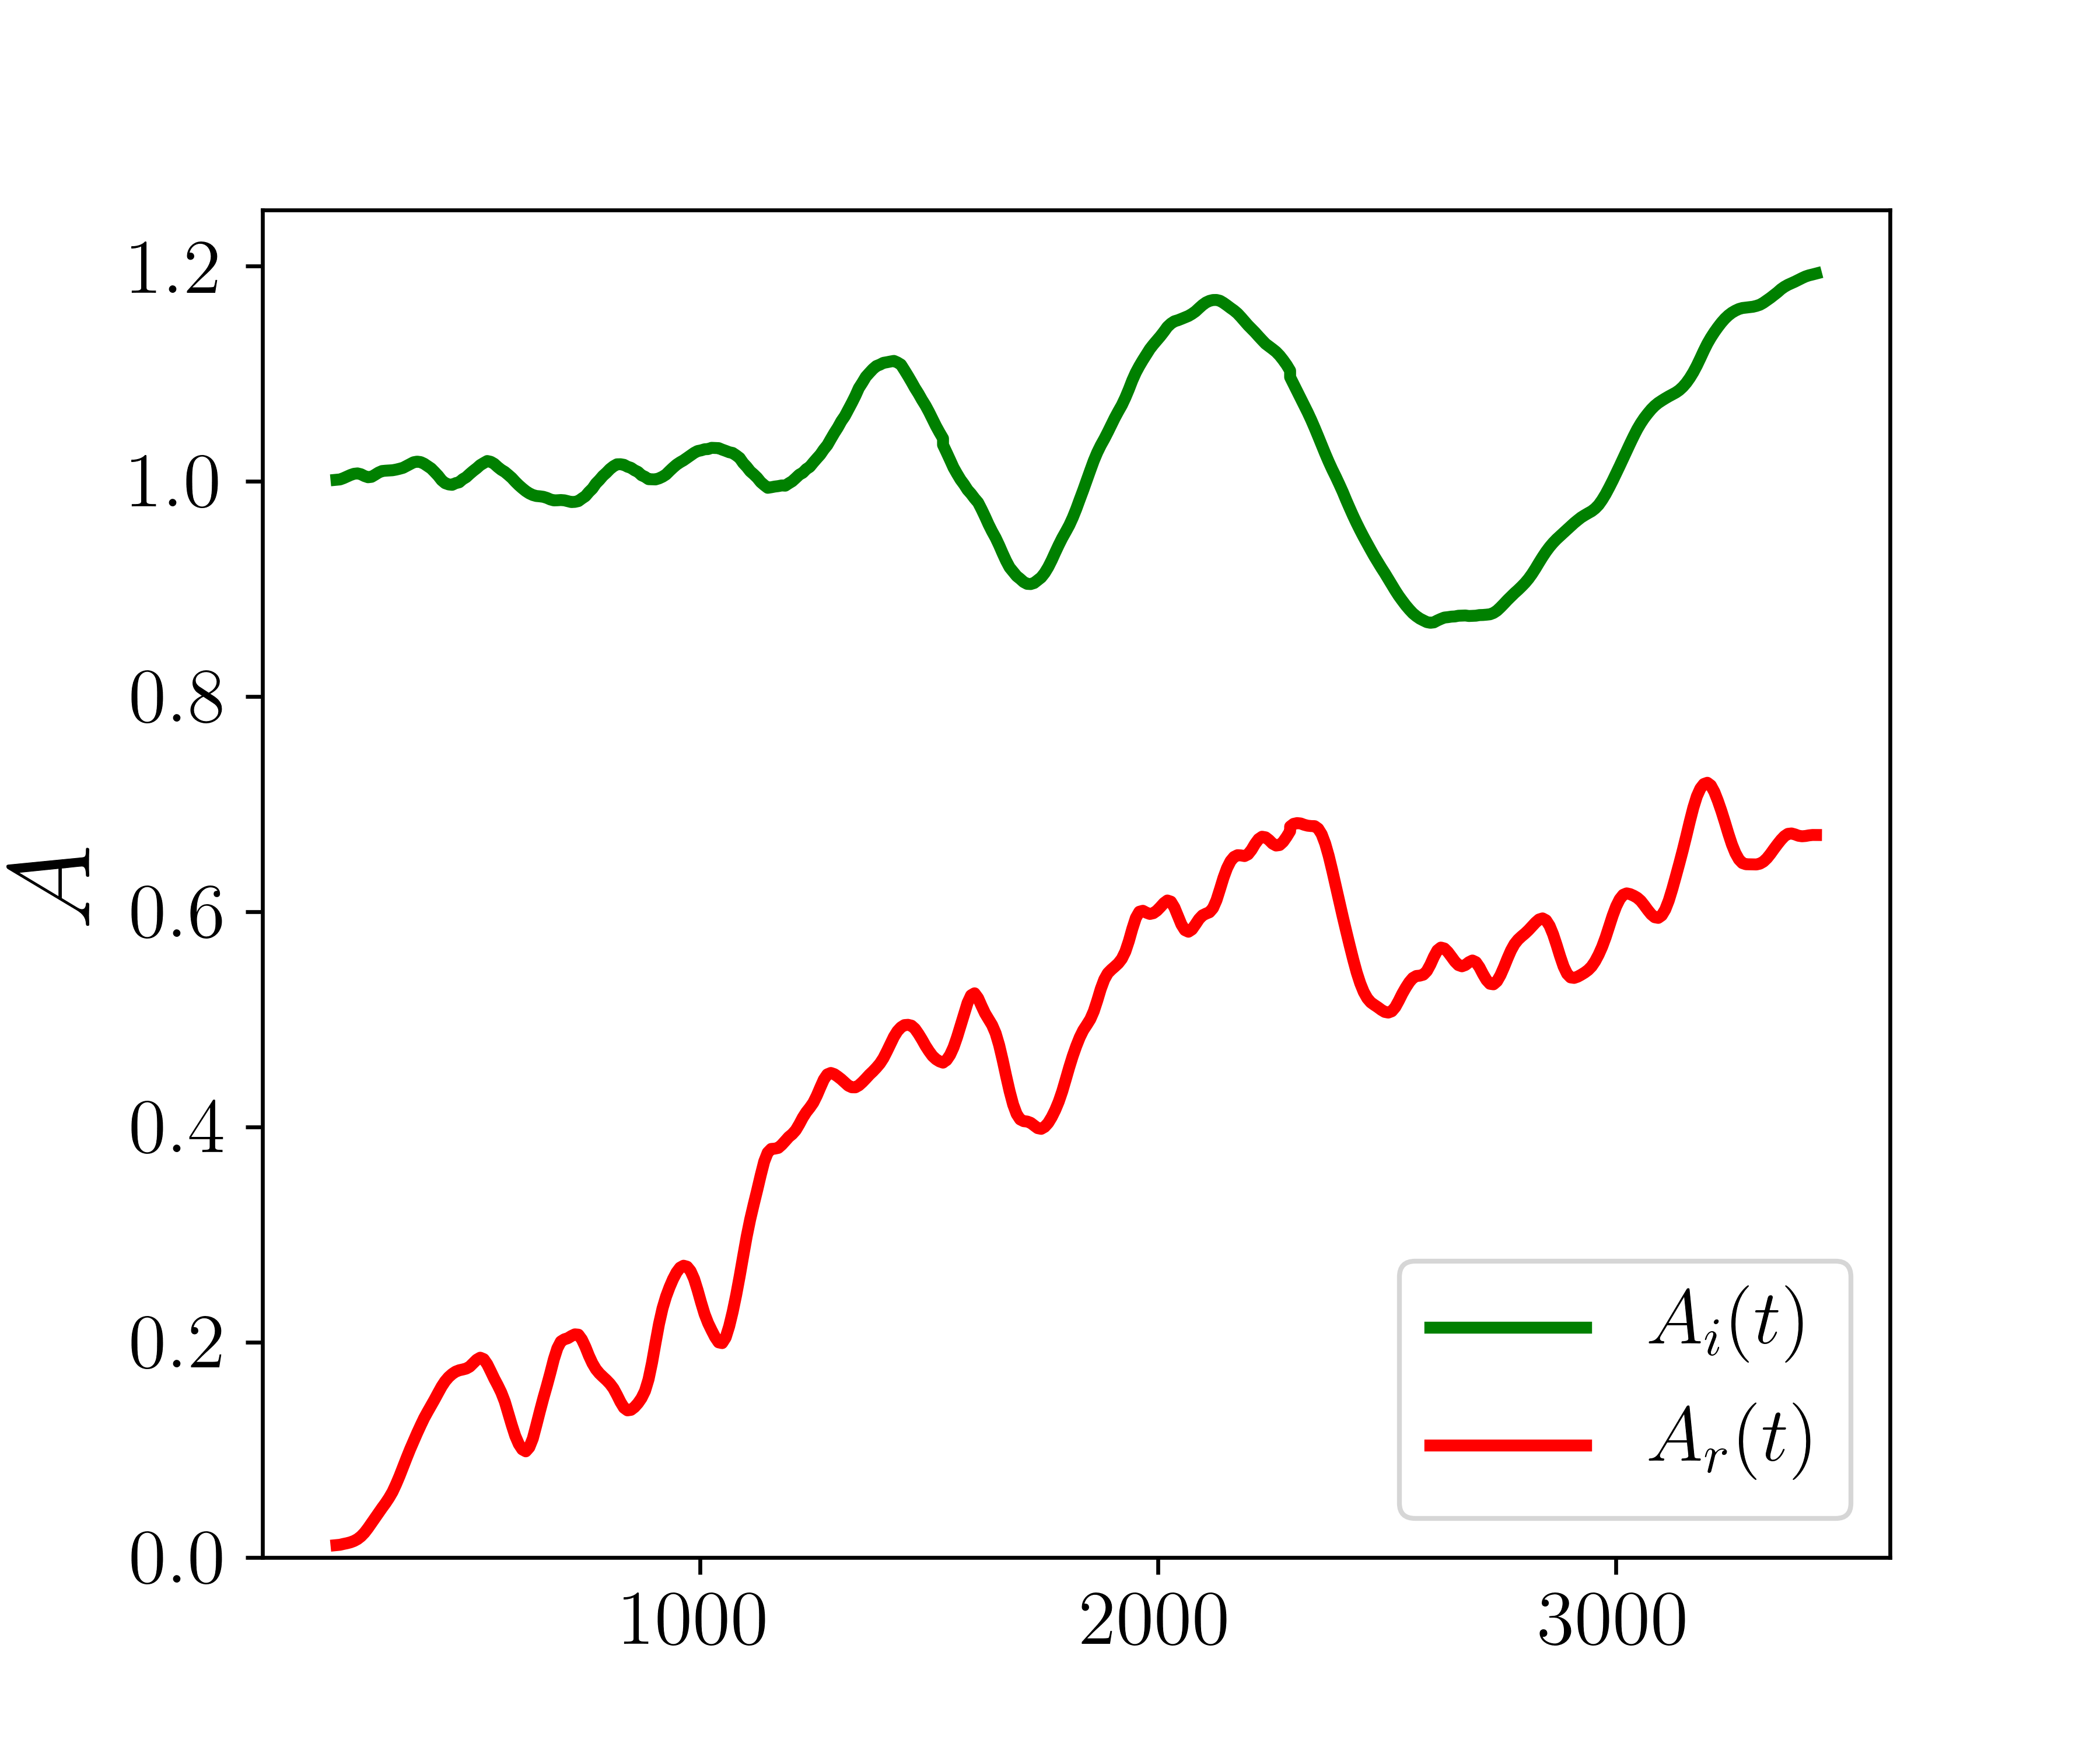
\includegraphics[width=0.8\columnwidth]{plots/nl_f_amps.png}
    \caption{The top panel shows the incident wave amplitude $A_i(t)$ (green)
    and the reflected wave amplitude $A_r(t)$ (red) just above the forcing zone.
    The bottom panel shows the behavior of the four components of the horizontal
    momentum flux budget over time, in units of the analytical estimate
    \autoref{eq:S_lin}: (green) flux incident on the critical layer, (blue) flux
    absorbed by the critical layer, (red) flux reflected at the critical layer,
    and (black) flux inside the synchronized layer.}\label{fig:nl_f_amps}
\end{figure}

Using these measured quantities, we may make plots of $\mathcal{R}_A^2$,
$\hat{F}_r$, $\hat{F}_s$, which are provided in \autoref{fig:nl_f_refl}. A
comparison between $\mathcal{R}_A^2$ and $\hat{F}_r$ is appropriate as $F
\propto A^2$. Visual inspection suggests the three quantities have reached their
asymptotic values after $t \gtrsim 1750/N$. An observation may be made that in
general $\hat{F}_r \geq \mathcal{R}_A^2$; this conforms to the expectation
that reflected flux consists of the simple reflected mode and higher order modes
as well.

\begin{figure}
    \centering
    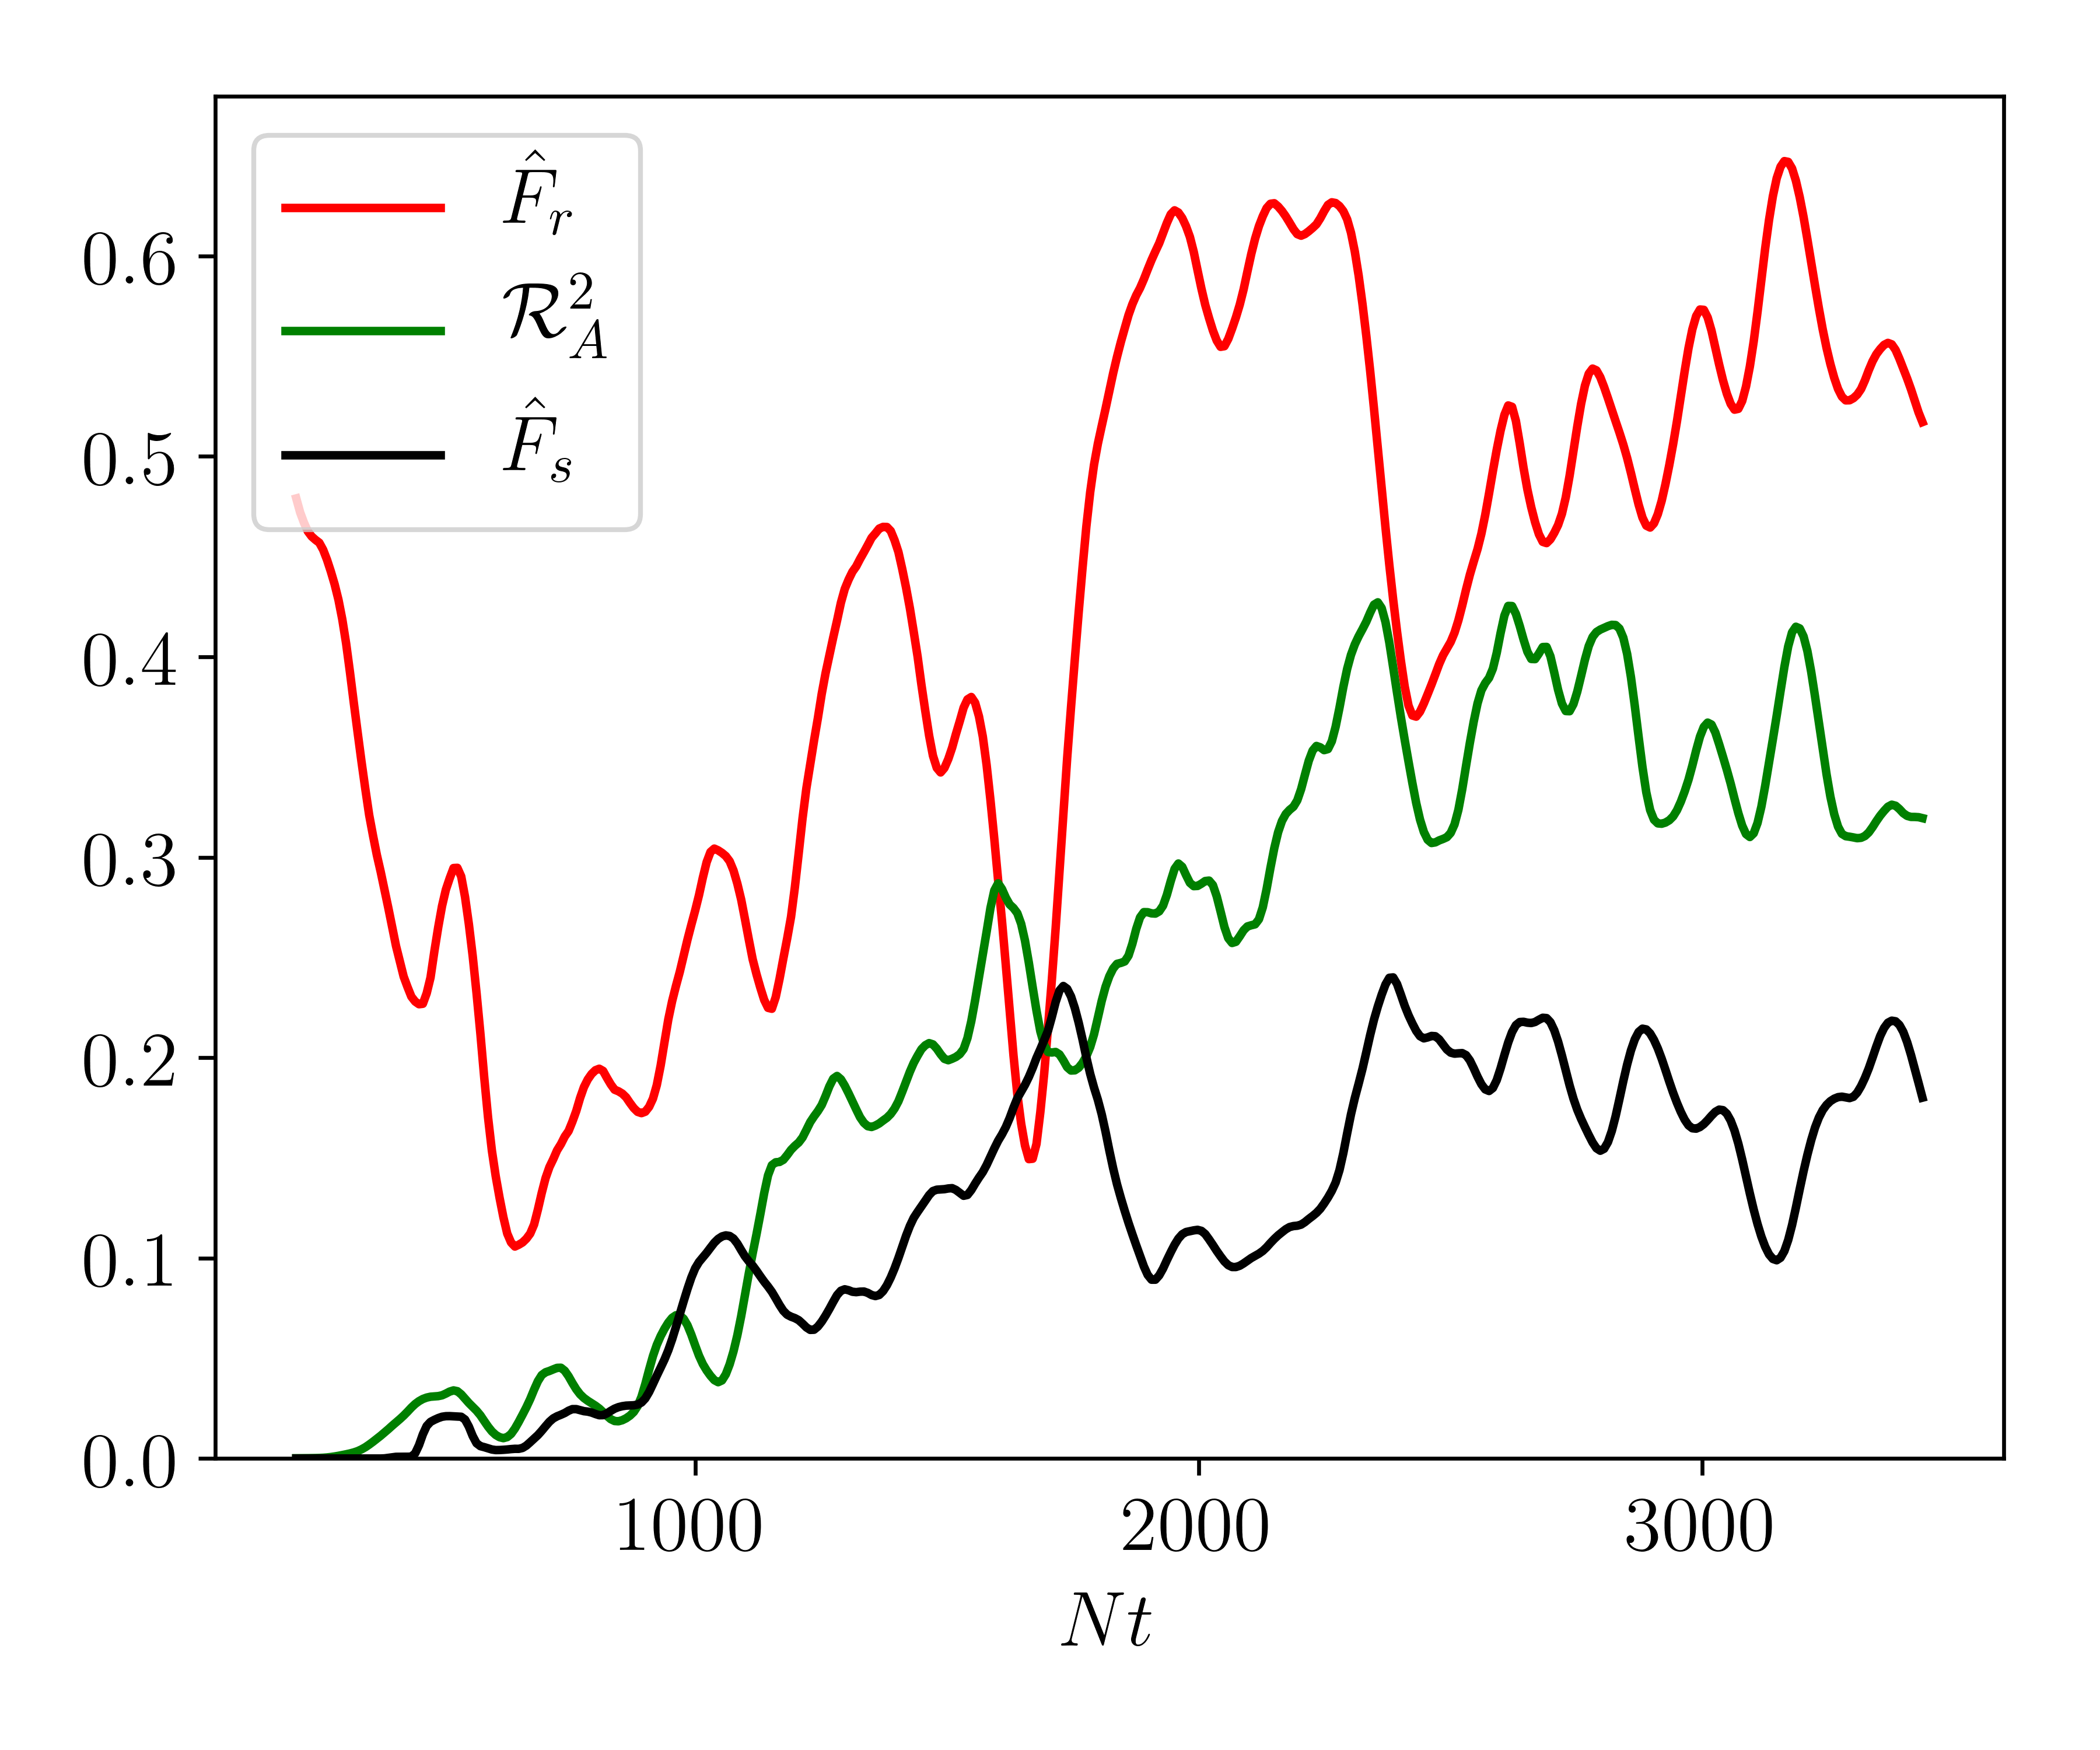
\includegraphics[width=\columnwidth]{plots/nl_f_refl.png}
    \caption{Behavior of $\mathcal{R}_A^2$, $\hat{F}_r$, and $\hat{F}_s$ as
    described by Equations~\ref{eq:Ra_def},~\ref{eq:srefl_def1},
    and~\ref{eq:srefl_def}. The coefficients seem to become comparatively stable
    past about $t = 1750/N$, indicating that an asymptotic value may have been
    reached.}\label{fig:nl_f_refl}
\end{figure}

\subsection{Resolution Study}\label{ss:convergence}

As the primary test of whether our simulations have obtained sufficient
resolution, we consider the convergence of $\mathcal{R}_A^2$, $\hat{F}_r$,
$\hat{F}_s$. Furthermore, we are able to compare our results against
\autoref{eq:crit_coeffs}, which appear to suggest that the behavior of incident
waves on the critical layer depends only on the local Richardson number (see
\autoref{s:khi} for details on our measurement of $\mathrm{Ri}$).

For each simulation in \autoref{tab:params}, we compute the median value of each
of $\mathcal{R}_A^2$, $\hat{F}_r$, $\hat{F}_s$, and $\mathrm{Ri}$ over the last
$1/4$ of simulation times from each simulation, where all simulations temporally
converged to what appeared to be asymptotic values. The bars show the temporal
variation of each measurement between the $16\%$ and $84\%$ range. We illustrate
the behavior of these averages at different $\mathrm{Re}$ in \autoref{fig:agg}.
\begin{figure}
    \centering
    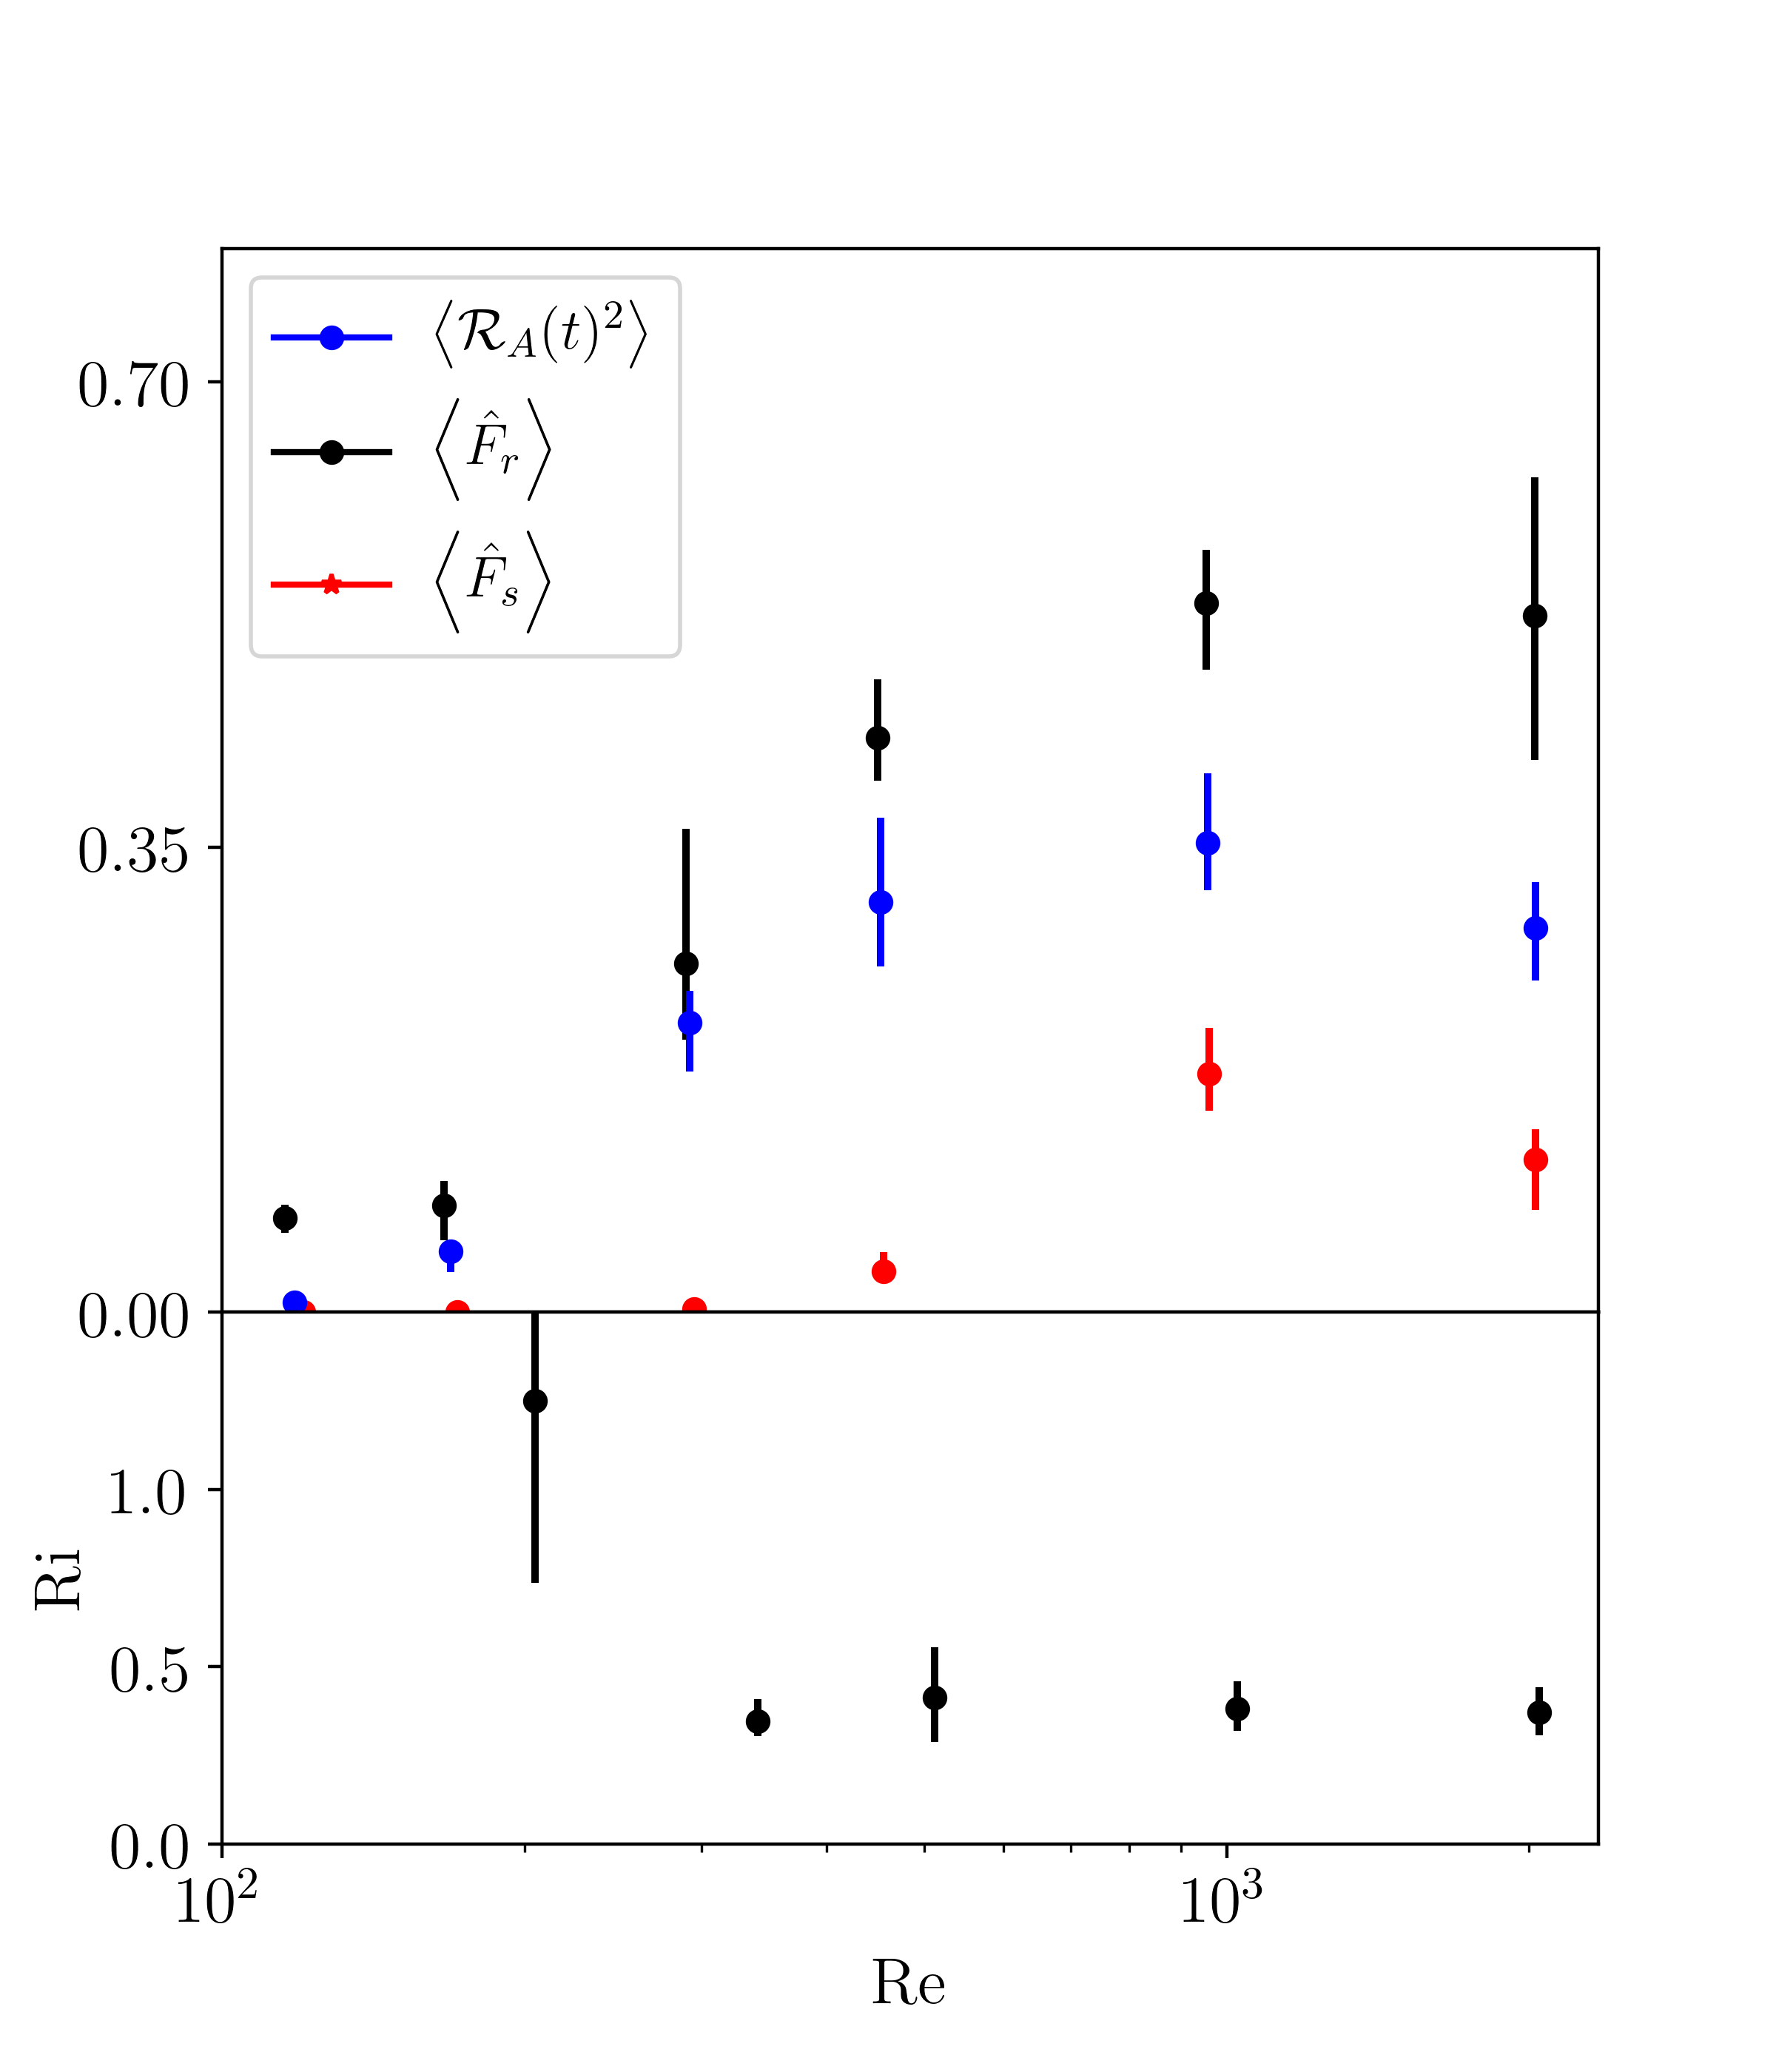
\includegraphics[width=\columnwidth]{plots/agg.png}
    \caption{Convergence of median $\hat{F}_r$, $\mathcal{R}_A^2$, $\hat{F}_s$,
    and $\mathrm{Ri}$ across runs with varying resolution and viscosity as given
    in \autoref{tab:params}. The bars show the temporal variation of each
    measurement between the $16\%$ and $84\%$ range. Small horizontal
    displacements are made for data points at identical $\mathrm{Re}$ for
    readability. Note that simulations with larger $\mathrm{Re}$ and resolution
    correspond to smaller viscosity and are more physically realistic. Our
    measurements seem to converge at large $\mathrm{Re}$. At the smallest
    $\mathrm{Re}$ value, $\mathrm{Ri} \approx 50$ is too large to fit on the
    plot.}\label{fig:agg}
\end{figure}

It is apparent that the Richardson number rapidly converges to $\mathrm{Ri}
\approx 0.4$ but the non-absorption measures converge more slowly. This is in
disagreement with \autoref{eq:crit_coeffs} calculated via the linear analytical
theory. This tension is natural: fluid motion within the critical layer is
turbulent, so transmission/reflection at the critical layer cannot be captured
by any linear calculation.

\section{Summary and Discussion}\label{s:discussion}

In this paper, we have performed numerical simulations of breaking IGWs in a
2D idealized WD fluid. We observe spontaneous formation of a critical layer that
separates a synchronized upper layer of fluid and a lower layer of fluid with no
mean horizontal flow. This critical layer then propagates downwards as a
continuous train of IGW are incident on it (see \autoref{fig:snapshots} for
snapshots from a fiducial simulation). Our primary conclusions regarding the
evolution of the critical layer are as follows:
\begin{itemize}
    \item The critical layer propagates downward by partially absorbing incident
        flux supplied by the continuous train of IGW, eventually spinning up the
        entire fluid (see \autoref{fig:nl_fluxes} for the time evolution of the
        mean flow and momentum flux in the fluid).

    \item \autoref{fig:nl_front} shows that the height of the critical layer
        $z_c(t)$ can be estimated from \autoref{eq:zc_anal}. The critical layer
        only absorbs $\sim 70\%$ of the incident flux in most simulations (see
        \autoref{fig:agg} for convergence at high resolutions).

        Note this absorbed fraction of incident momentum flux we
        measure differs from both analytical \citep{booker_bretherton} and
        numerical \citep{barker_ogilvie} results in the existing literature. The
        former result is a linear calculation and is superceded by our nonlinear
        simulation; we speculate on our discrepancy with the latter in
        \autoref{ss:other} below.

    \item We compute the asymptotic amplitude of reflected waves off the
        critical layer as well as the average reflected momentum flux in
        \autoref{fig:nl_f_refl}. Also illustrated is the asymptotic value of an
        extra momentum flux just above the critical layer, likely responsible
        for momentum redistribution within the critical layer. Our simulations
        are run sufficiently long to be temporally converged.

    \item Finally, the largest flow variations are found within the turbulent
        critical layer, whose minimum width is set by the Kelvin-Helmholtz
        instability.
\end{itemize}
In the subsequent sections, we will discuss the validity of these results and
their application to astrophysical systems.

\subsection{Physical Sources of Dissipation in WDs}\label{ss:disp}

The most significant linear damping in WD g-modes comes from radiative damping
\citep{fullerI}. In \citep{wu} and \citep{fullerI}, the radiative damping rate
is given in terms of $\omega_i = \gamma \omega_r$, where $\omega_r$ is the
frequency of the g-mode. Typical values for $\gamma$ range from $10^{-4}$ to
$10^{-11}$ depending on $n$ of the g-mode.

We will assume this prescription directly transfers to propagating IGW, which
results in general agreement with \citep{bukart}'s estimate of radiative damping
rates. Then, making coarse identification $\omega_i \sim \nu k^2 \approx \nu
k_z^2$, we find that $\mathrm{Re} \sim \frac{1}{\gamma}$. Even at $\gamma =
10^{-4}$ however, the corresponding $\mathrm{Re}$ is far too weak to suppress
reflection/transmission at the critical layer (e.g.\ \autoref{fig:agg}).

Another source of dissipation considered in \citep{bukart} is turbulent
conbmtive damping. They find this damping rate to never exceed that of
radiative damping, and so it is also too weak to suppress critical layer
formation in our problem.

Finally, we consider the impact of magnetic winding. In \citep{bukart}, magnetic
winding is used to enforce solid body rotation on the grounds that $t_A \gg
t_{gw}$, where
\begin{equation}
    t_A = \int\limits_0^R \frac{\sqrt{4\pi \rho}}{B_0}\;\mathrm{d}r
        \sim 10^2\;\mathrm{yr}\p{\frac{10^3\;\mathrm{G}}{B}},
\end{equation}
the Alfv\'en wave crossing time (evaluated for a CO WD in \citealp{fullerIV}),
measures the magnetic coupling time and $t_{gw}$ measures the gravitational wave
inspiral timescale. Before solid body rotation is attained, another relevant
timescale is the synchronization timescale $t_s$. For a tidal torque $\tau$ and
tidal forcing frequency $\sigma = m\p{\Omega - \Omega_{spin}}$, we note that
angular momentum transfer is $\pd{M_{sync}}{t} \sigma R^2 = \tau$, where
$M_{sync}$ denotes the mass of the WD that has synchronized. Thus, the
synchronization timescale is
\begin{align}
    t_{sync} &\sim \frac{M_{sync}\sigma R^2}{\tau},\\
        &\sim 20\;\mathrm{yr}
            \p{\frac{M_{sync}}{10^{-4}M_{\odot}}}
            \p{\frac{\sigma}{2\pi / (1\;\mathrm{hr})}}
            \p{\frac{R}{R_{\oplus}}}^2
            \p{\frac{10^{-14} GM_{\odot}^2/R_{\oplus}}{\tau}}.
\end{align}
A representative $\tau$ has been taken from \citep{bukart}. Only $M_{sync} \sim
10^{-4}M_{\odot}$ need be heated for the thermodynamically interesting effects
studied in \citep{fullerIV} and \citep{tidal_novae}, it seems that strong shear
flows may exist even in the presence of magnetic coupling.

\subsection{Applicability to Astrophysical Systems}\label{ss:other}

Below, we speculate on the applicability of our results to general astrophysical
problems of interest:
\begin{itemize}
    \item In astrophysical systems, $k_{\perp} \ll k_r$, while in our study,
        $k_x \simeq k_z$. True turbulence is expected to be isotropic at small
        scales, which may introduce different behavior for different ratios of
        $k_z/k_x$. However, $k_x \ll k_z$ is a numerically difficult regime; we
        defer its exploration to future work.

    \item In~\cite{barker_ogilvie}, inwards-propagating IGW are excited that
        break via geometric focusing. They find no reflected wave despite their
        nonlinear timescales being $10\times$ shorter than their viscous
        timescale, in contrast with the reflective behavior observed in our
        simulations. It is plausible the discrepancy arises due to the differing
        causes of wave breaking (geometric focusing vs.\ density
        stratification), but their simulations are also at significantly higher
        artificial viscosities than ours, as we show below.

        Associating $t_{L} \sim \nu k^2 \approx \nu k_z^2$ with the visocus
        timescale and $t_{NL} \sim \bm{u} \cdot \bm{\nabla} \sim \omega$ for the
        nonlinear timescale, we find their $\lambda = \frac{t_{NL}}{t_L} \sim
        \mathrm{Re}$ our Reynolds number. Our simulations indicate $\mathrm{Re}
        \gtrsim 500$ are required to observe the correct asymptotic behavior in
        terms of horizontal momentum flux reflection/transmission, so it is
        possible their lack of reflection is resolution limited.

    \item Our results give some tentative understanding of where tidal heating
        is expected to occur. While we use a barotropic equation of state and do
        not track heat deposition, we can recall that the strongest small-scale
        variations in fluid flow are localized within the critical layer. Thus,
        we posit that a substantial fraction of the energy carried by the IGW is
        deposited in the very narrow critical layer. Then, as the critical layer
        propagates downwards, the entire star is heated. This tidal heating
        model differs flom that used in \citep{tidal_novae}, and its effects
        will be studied in future work.
\end{itemize}

\section{Acknowledgements}\label{s:ack}

This work has been supported in part by NASA FINESST grant
19-ASTRO19-0041.%chktex 8

\bibliographystyle{mnras}
\bibliography{Su_IGW_break}

\clearpage
\onecolumn
\appendix

\section{Forcing Solution}\label{s:force_solved}

To solve for the excited wave amplitude in the linear problem, consider the
complexified linearized system of equations, then $\pd{}{t} \to -i\omega,
\pd{}{x} \to ik_x$. Assuming all fields have dependence $u_z(x, z, t) =
\tilde{u_z}(z) e^{ik_xx - i\omega t}$ and dropping the tildes for convenience,
this gives:
\begin{align*}
    \rd{u_{z}}{z} + ik_xu_x &= 0,\\
    -i\omega u_x + ik_x \varpi + gHik_x \Upsilon &= 0,\\
    -i\omega u_{z} + \rd{\varpi}{z} + gH\rd{\Upsilon}{z}
        - \frac{\varpi}{H} &= 0,\\
    -i\omega \Upsilon - \frac{u_{z}}{H} &=
        Ce^{-\frac{(z - z_0)^2}{2\sigma^2}}.
\end{align*}
We have replaced all partial derivatives with regular derivatives. This can be
recast solely in terms of $u_{z}$ as
\begin{align*}
     \rtd{u_{z}}{z} - k_x^2u_{z} - \frac{1}{H}\rd{u_{z}}{z}
        + u_{z}\frac{N^2k_x^2}{\omega^2} &=
    -\frac{gk_x^2}{\omega^2}Ce^{-\frac{(z - z_0)^2}{2\sigma^2}}
        .\label{eq:narrow_inhomo}
\end{align*}
The homogeneous solutions are of form $u_{z,\pm}(z) = e^{\p{\frac{1}{2H} \pm
ik_z}\p{z - z_0}}$ where $k_z$ satisfies the dispersion relation
\autoref{eq:disp_rel}. We compute the solution to the inhomogeneous ODE by the
method of variation of parameters. The Wronskian can be computed
\begin{equation}
    W \equiv \det \begin{vmatrix}
        u_{z,+} & u_{z,-} \\[4pt]
        \rd{u_{z,+}}{z} & \rd{u_{z,-}}{z}
    \end{vmatrix} = -2ik_ze^{z/H}.
\end{equation}
The general solution is then
\begin{equation}
    u_z = -u_{z,+}\int \frac{1}{W} u_{z,-} \p{-\frac{gk_x^2}{\omega^2}
            Ce^{-\frac{(z - z_0)^2}{2\sigma^2}}}\;\mathrm{d}z
        + u_{z,-}\int \frac{1}{W} u_{z,+} \p{-\frac{gk_x^2}{\omega^2}
            Ce^{-\frac{(z - z_0)^2}{2\sigma^2}}}\;\mathrm{d}z.
\end{equation}
Taking these integrals and applying boundary conditions $u_z\p{z \to \infty} =
u_{z,+}, u_z\p{z \to -\infty} = u_{z,-}$ gives exact solution
\begin{equation}
    u(z) = \frac{C}{2ik_z}\frac{gk_x^2}{\omega^2}
            e^{\frac{\p{\frac{\sigma^2}{2H} \pm ik_z\sigma^2}^2}{2\sigma^2}}
                \sqrt{2\sigma^2} \frac{\sqrt{\pi}}{2}\s{
                    -u_+\p{1 + \erf\p{\xi}}
                    + u_- \p{\erf\p{\xi} - 1}}
\end{equation}
If we are concerned with only $z$ scales significantly larger than $\sigma$,
then we may take $\erf(\xi) \approx \Theta(\xi)$. If we further assume $k_zH \gg
1$ and restore the $e^{ik_xx - i\omega t}$ factor, we recover the cited form
\autoref{eq:uz_lin}
\begin{equation}
    u_{z}(x, z, t) = -\frac{C}{2ik_z}\frac{gk_x^2}{\omega^2}
        e^{-\frac{k_z^2\sigma^2}{2}}
        \sqrt{2\pi \sigma^2} e^{ik_xx - i\omega t} \times
    \begin{cases}
        e^{\p{\frac{1}{2H} + ik_z}\p{z - z_0} + \frac{k_z\sigma^2}{2H}}
            & z > z_0,\\
        e^{\p{\frac{1}{2H} - ik_z}\p{z - z_0} - \frac{k_z\sigma^2}{2H}}
            & z > z_0.
    \end{cases}
\end{equation}
We use the plane wave approximation in our fitting routines since we generally
fit many $\sigma$ away from $z_0$, and orthogonality with other modes is
essential for a reliable fit.

\section{Kelvin-Helmholtz Instability and Critical Layer Width}\label{s:khi}

The observation of reflected/transmitted waves is in accordance with previous
studies as discussed in \autoref{ss:wave_breaking}. Studies have shown that a
local Richardson number $\mathrm{Ri} \sim 1/4$ corresponds to the onset of
reflectivity. This $\mathrm{Ri}$ also corresponds to the onset of the
Kelvin-Helmholtz instability (KHI). Indeed, in our simulations, visual
inspection suggests the KHI is present in the critical layer (see
\autoref{fig:snapshots}). It is natural to suspect then that the shear flow
cannot steepen any further than KHI onset. To verify this, we compute a local
$\mathrm{Ri}$ for the shear flow around the critical layer.

Since fluid instabilities are local, $\mathrm{Ri}$ must be measured in the
immediate vicinity of a fluid parcel. Thus, we first assign an $\mathrm{Ri}$ for
every $x$ in the critical layer, then take the median as $\mathrm{Ri}$ for the
entire layer. To avoid noisiness, the local $\mathrm{Ri}$ is computed using the
vertical distance over which the local $u_x$ increases from $0.3 \times$ its
critical value to its critical value. The value $0.3$ is necessary to exclude
the small mean flow generated in the weakly nonlinear regime well below the
critical layer. This is written
\begin{align}
    z_{CL, \min}(x, t) &\equiv \argmin_z
        \z{z\mid u_x(x, z, t) > 0.3\overline{U}_c},\\
    z_{CL, \max}(x, t) &\equiv \argmax_z
        \z{z\mid u_x(x, z, t) < \overline{U}_c},\\
    \mathrm{Ri}(t) &\equiv
        \med_x\p{\frac{N^2 \p{z_{CL, \max} - z_{CL, \min}}^2}{(0.7
            \overline{U}_c)^2}}.\label{eq:ri_med_def}
\end{align}
To understand the variation in $\mathrm{Ri}$ over $x$, we can also plot using
the minimum over $x$ (the maximum is significantly noisier). Both of these are
shown in \autoref{fig:nl_f_ri}. The critical layer quickly narrows to its
minimum width, driven by the anti-diffusivity of IGWs.
\begin{figure}
    \centering
    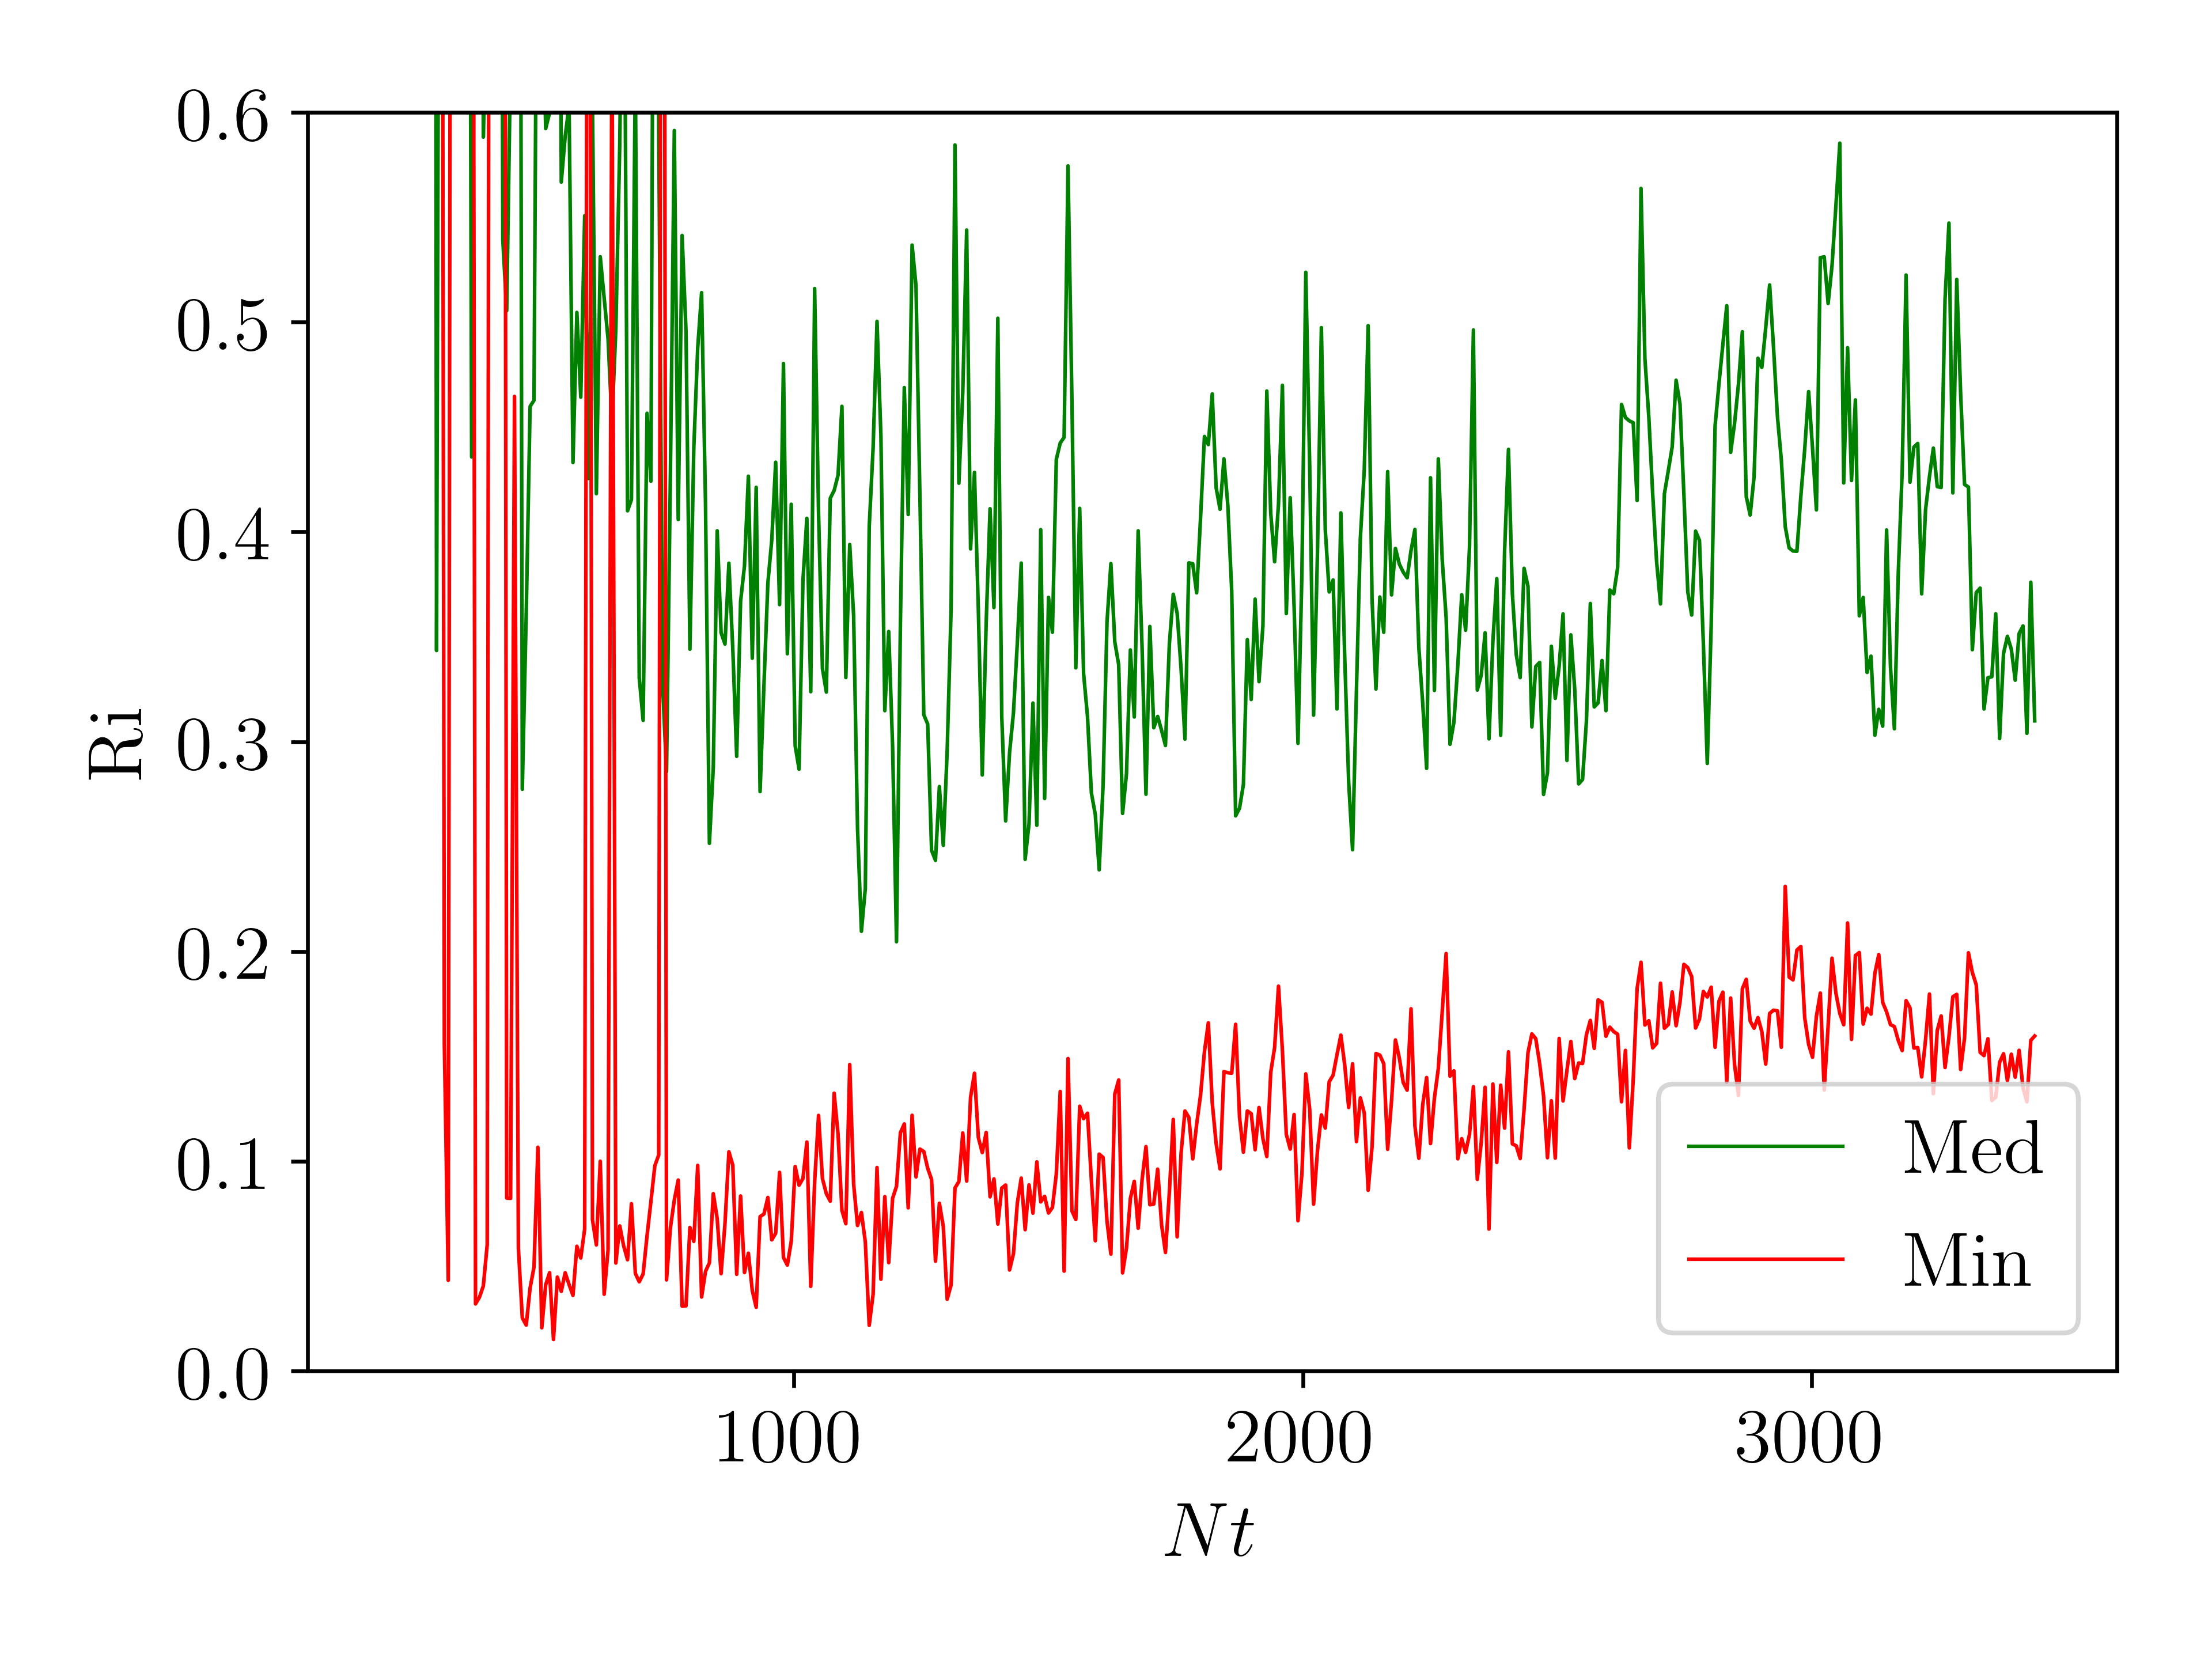
\includegraphics[width=0.6\columnwidth]{plots/nl_f_ri.png}
    \caption{Local Richardson number of the flow at the critical layer over time
    as defined in \autoref{eq:ri_med_def}. The red and solid green lines denote
    respectively the minimum and median of $\mathrm{Ri}$ over $x$ (the maximum
    greatly exceeds the vertical scale of this plot). These numbers effectively
    measure the mean and spread in width of the critical layer over $x$. Note
    that $\mathrm{Ri} \sim \frac{1}{4}$ corresponds to the KHI, so this plot
    suggests the shear at the critical layer does not steepen past the KHI
    onset.}\label{fig:nl_f_ri}
\end{figure}

\section{Equation Implementations}\label{se:strat_impl}

We denote $x \in [0, L_x], z \in [0, L_z]$ the simulation domain and $N_x, N_z$
the number of spectral modes in the respective dimensions.

Numerically, the nonlinear $\frac{\bm{\nabla}P}{\rho}$ term is problematic: we
desire a system where the fluid fields are not divided by one another. We
introduce $\varpi = \frac{P}{\rho}$ instead, then mandate $\overline{\rho},
\overline{\varpi}$ background fields satisfy hydrostatic equilibrium
$\bm{\nabla}\overline{\varpi} + \overline{\varpi} \bm{\nabla}\overline{\rho} +
g\uv{z} = 0$. Taking isothermal stratification, we find $\overline{\varpi} = gH$. We
further change variables to $\Upsilon = \ln \rho - \ln \overline{\rho}$ and
$\varpi' = \varpi - \overline{\varpi}$ deviations from the background state to
obtain a system of equations at most quadratic in fluid fields:
\begin{subequations}\label{se:nl_var}
    \begin{align}
        \bm{\nabla} \cdot \bm{u} &= 0,\\
        \pd{\Upsilon}{t} + \p{\bm{u} \cdot \bm{\nabla}} \Upsilon
            - \frac{u_z}{H} &= 0,\\
        \pd{u_{x}}{t} + \p{\bm{u} \cdot \bm{\nabla}}u_{x}
            + \pd{\varpi'}{x} + gH\pd{\Upsilon}{x}
            + \varpi' \pd{\Upsilon}{x} &= 0,\\
        \pd{u_z}{t} + \p{\bm{u} \cdot \bm{\nabla}}u_z
            + \pd{\varpi'}{z} + gH\pd{\Upsilon}{z}
            + \varpi' \pd{\Upsilon}{z} - \frac{\varpi'}{H} &= 0.
    \end{align}
\end{subequations}
It bears noting that these equations are exactly equivalent to the original
Euler equations and hence conserve horizontal momentum.

\subsection{Artificial Dissipation}

The nonlinear terms in the above equations will transfer energy from lower
wavenumbers to higher wavenumbers. Since spectral codes have no numerical
dissipation, artificial dissipation must be added. To ensure the dissipitive
system conserves horizontal momentum exactly, we begin by adding dissipitive
terms to the flux-conservative form of the Euler fluid equations
\autoref{se:nl_orig} (we use stress tensor $\tau_{ij} = P\delta_{ij}$):
\begin{subequations}
    \begin{align}
        \bm{\nabla} \cdot \bm{u} &= 0,\\
        \partial_t \rho + \bm{\nabla} \cdot (\rho \bm{u} - \nu
            \bm{\nabla}(\rho - \overline{\rho})) &= 0,\label{eq:visc_cons_mom}\\
        \partial_t (\rho \bm{u}) + \bm{\nabla} \cdot (\rho \bm{u} \bm{u}
            + \mathrm{diag}(\rho \varpi)
            - \nu \rho \bm{\nabla}\bm{u})
            + \rho g \uv{z} &= 0.
    \end{align}
\end{subequations}
The same $\nu$ is used for both the diffusive and viscous term, though this is
not required. Since the dissipation is not physical and is purely used for
numerical stability, we choose it such that hydrostatic equilibrium is not
modified (hence $\nu$ acts only on $\rho - \overline{\rho}$).

One last consideration we found necessary was masking out nonlinear terms in the
forcing zone with a similar form to \autoref{eq:Gamma}. In the absence of this
mask, a strong mean flow localized to the forcing zone developed. The mask used
was
\begin{equation}
    \Gamma_{NL}(z) = \frac{1}{2}\s{2
        + \tanh \frac{z - (z_0 + 8\sigma)}{\sigma}
        - \tanh \frac{z - z_B}{\sigma}}.
\end{equation}

Including the damping layers and forcing terms as described in
\autoref{s:numerics}, we finally obtain the full system of equations as
simulated in Dedalus:
\begin{subequations}\label{se:dedalus_eqs}
    \begin{align}
        \bm{\nabla} \cdot \bm{u} ={}& 0,\\
        \partial_t \Upsilon - \frac{u_z}{H}
            ={}& -\Gamma(z) \Upsilon
                + \frac{F}{\overline{\rho}(z)}e^{-\frac{(z - z_0)^2}{2\sigma^2}}
                    \cos \p{k_xx - \omega t}\nonumber\\
            & + \Gamma_{NL} \bigg[-\p{\bm{u} \cdot \bm{\nabla}}\Upsilon
                + \nu\p{\nabla^2 \Upsilon + \p{
                    \bm{\nabla} \Upsilon} \cdot \p{\bm{\nabla}\Upsilon}
                    - \frac{2}{H}\partial_z \Upsilon
                    + \frac{1 - e^{-\Upsilon}}{H^2}}\bigg],\\
        \pd{u_x}{t} + \pd{\varpi'}{x} + gH\pd{\Upsilon}{x} ={}&
            -\Gamma(z) u_x
            + \Gamma_{NL}\bigg[\nu \nabla^2 u_x
            - u_x \nu\p{\nabla^2 \Upsilon + \p{\bm{\nabla} \Upsilon} \cdot
                \p{\bm{\nabla}\Upsilon} - \frac{2}{H}\partial_z \Upsilon
                + \frac{1 - e^{-\Upsilon}}{H^2}}\nonumber\\
            &+ 2\nu \p{\p{\p{\bm{\nabla}\Upsilon} \cdot \bm{\nabla}}u_x
                - \frac{1}{H}\partial_z u_x}
                - \p{\bm{u} \cdot \bm{\nabla}}u_x
                - \varpi' \pd{\Upsilon}{x}\bigg],\\
        \pd{u_z}{t} + \pd{\varpi'}{z} + gH\pd{\Upsilon}{z} - \frac{\varpi'}{H}
            ={}& -\Gamma(z) u_z
            +\Gamma_{NL}\bigg[\nu \nabla^2 u_z
            - u_z \nu\p{\nabla^2 \Upsilon + \p{\bm{\nabla} \Upsilon} \cdot
                \p{\bm{\nabla}\Upsilon} - \frac{2}{H}\partial_z \Upsilon
                + \frac{1 - e^{-\Upsilon}}{H^2}}\nonumber\\
            &+ 2\nu \p{\p{\p{\bm{\nabla}\Upsilon} \cdot \bm{\nabla}}u_z -
                \frac{1}{H}\partial_z u_{z}}
            - \p{\bm{u} \cdot \bm{\nabla}}u_z
            - \varpi' \pd{\Upsilon}{z}\bigg].
    \end{align}
\end{subequations}
\label{lastpage} % chktex 24
\end{document}
